\documentclass[10pt,a4paper,twocolumn]{article}
\usepackage[a4paper,margin=17mm,columnsep=6mm]{geometry}
\usepackage[T1]{fontenc}
\usepackage{newtxtext,newtxmath}
\usepackage{microtype}
\usepackage{amsmath}
\usepackage{booktabs}
\usepackage{graphicx}
\usepackage{xcolor}
\usepackage[font=small,labelfont=bf,skip=4pt]{caption}
\usepackage{enumitem}
\usepackage[hidelinks]{hyperref}
\usepackage{tabularx}
\usepackage{array}
\usepackage{longtable}
\setlist{nosep,leftmargin=*}
\graphicspath{{fig/}}
\newcommand{\Npass}{290}\newcommand{\Nmiss}{27}\newcommand{\Nchecks}{317}\newcommand{\Nreported}{26}\newcommand{\Nstationtests}{16}\newcommand{\Nfitted}{8}
\newcommand{\NFpass}{26}\newcommand{\NFmiss}{2}
\newcommand{\NPpass}{18}\newcommand{\NPmiss}{10}
\newcommand{\NMpass}{16}\newcommand{\NMmiss}{7}
\newcommand{\NDpass}{195}\newcommand{\NDmiss}{7}
\newcommand{\NGpass}{35}\newcommand{\NGmiss}{1}
\newcommand{\Nkindopen}{4}
\newcommand{\Nkindother}{11}
\newcommand{\Nkindsource}{7}
\newcommand{\Nkindsources}{5}
\newcommand{\FgLandWeight}{26334}
\newcommand{\FgLandPast}{5439}
\newcommand{\FgLandModel}{5598}
\newcommand{\FgCamPoint}{0.13}
\newcommand{\FgCamShip}{0.04}
\newcommand{\FgAirHLo}{19973}
\newcommand{\FgAirHHi}{20013}
\newcommand{\FgAirVLo}{149.5}
\newcommand{\FgAirVHi}{150.8}
\newcommand{\FgAirBank}{0.46}
\newcommand{\FgHudHorizon}{0.26}
\newcommand{\Ncommit}{d8758f7}\newcommand{\Ndate}{2026-11-13 19:59}

\renewcommand{\arraystretch}{1.08}
\setlength{\tabcolsep}{4pt}
\raggedbottom
\renewcommand{\topfraction}{0.92}\renewcommand{\dbltopfraction}{0.92}\renewcommand{\bottomfraction}{0.6}
\renewcommand{\textfraction}{0.06}\renewcommand{\floatpagefraction}{0.85}\renewcommand{\dblfloatpagefraction}{0.85}
\setcounter{topnumber}{3}\setcounter{dbltopnumber}{3}\setcounter{totalnumber}{5}
\makeatletter\setlength{\@fptop}{0pt}\setlength{\@dblfptop}{0pt}\makeatother
\begin{document}

\twocolumn[
\begin{@twocolumnfalse}
\begin{center}
{\LARGE\bfseries Flight Dynamics of the Global Hawk in JSBSim\par}
\vspace{6pt}
{\large\bfseries A model of the RQ-4A from public data, calibrated on NASA's flight records, with its own flight laws and a ground control station\par}
\vspace{10pt}
{\large Technical report \quad\textbullet\quad November 2026\par}
\vspace{10pt}
\end{center}
\begin{abstract}
\noindent
A flight-dynamics model of the Global Hawk that NASA flew as N872NA, an RQ-4A, has been written in JSBSim for the FlightGear simulator, together with
the flight laws that fly it and a ground control station that commands it. Neither the manufacturer's aerodynamic data, nor an engine deck, nor the real
flight control laws are public. The model is therefore built from published dimensions and weights, NASA's drawing and 3-D model, the tunnel test of
its wing section, the certification databank of its engine family, and the flight records NASA published from the ATTREX campaigns, which carried a
meteorological system that logged attitude, angle of attack, Mach number and pressure on 26 flights. The wing is 80 strips on a lifting line with
section data; the engine is a cycle model of the AE~3007 family, proved first on the Citation~X's variant. With the flat rating read as one limit on
turbine temperature, nothing fitted, the climb from 10\,000 to 40\,000\,ft comes out 4 to 11\,\% slow against the two measured flights; one drag
increment and a 1\,\% change of the fan-speed limit, fitted to the climb above 40\,000\,ft and the cruise-climb together, hold the cruise-climb within 890\,ft for 20 hours, with the CFD's rise of the section's drag with Mach number in the tables, and leave the time to 55\,000\,ft
9.0\,\% short of the flights' (a miss; the limit was 5). The trimmed lift-curve slope is 2.8\,\% over the flights' at Mach~0.52 and 15.5\,\% at Mach~0.6 (a miss that comes from the added drag), the take-off within
13\,\%, and the approach of a second recorded landing is predicted from a spoiler setting fitted on the first. The endurance, flown to the
65\,000\,ft that NASA gives as the ceiling, comes out at 34.9\,h, from the physics and fitted to nothing; the published figures it can be set beside
(NASA's ``31+'', the RQ-4A's official record of 30\,h 24\,min, later blocks' 33 to 35\,h) are capabilities and records with unknown reserves and
payloads, so they are a sanity window, not a target; without the ceiling the model climbs past it and reaches 35.1\,h. The wing section's pitching moment grows with Mach number faster in the section data than in the
tunnel, which one fitted exponent corrects, and with it the bare airframe's speed mode at the cruise becomes stable. The flight laws are the author's design and are held to their own requirements only: they fly a mission
from stand to stand, the two recorded landings within 5\,KEAS and 0.5\,m/s of the records, a navigator failure of the kind that destroyed an RQ-4B in 2017, a
lost link, and a landing without the engine. In FlightGear the aircraft is flown through the station's link by the same logic.
Landings in gusts are flown in hundreds on a bench and in FlightGear: a stabilisation of the landing law lowers the hard landings where this aircraft lands hard, two airliners' rules of thumb for the
approach speed buy margin to the stall limit and pay for it in sink, runway and, for one of them, the structural limits, and the low wing's tips, which bend, set the limit on the bank at touchdown.
Limits were set before results and not moved: \Npass{} checks pass and \Nmiss{} miss. Only \NFpass{} of the passes are held to flight records, \Nfitted{} of them after
a fit to the same record; \NDpass{} are the laws and the software against the author's own requirements. Every miss is listed with its cause.
\end{abstract}
\vspace{6pt}
\end{@twocolumnfalse}
]

\section{Introduction}
The Global Hawk is a high-altitude, long-endurance unmanned aircraft: a wing of aspect ratio 25, one turbofan above the rear fuselage, a V-tail, and more
than half its take-off weight in fuel. NASA flew two early RQ-4As on science missions from 2010; one of them, N872NA, flew the ATTREX campaigns from 2011
to 2015 \cite{ov}. Nobody holds a stick: a mission computer flies a loaded plan through its own control laws, and crews on the ground command it, one
element for taxi, take-off and landing over a line-of-sight link, another for the mission over a satellite \cite{ops}.

This report describes a model of that aircraft for FlightGear \cite{fg}, and what it was checked against. It differs from the author's other
models in what could be known. No wind-tunnel or CFD data of the aircraft is public, no engine map, no flight manual, and nothing of the control laws
beyond how the aircraft is seen to fly. What is public is unusual: 420 hours of flight records, most of them at 20\,Hz. The model is built up from first
principles and published geometry and then held to those records; the laws and the ground station are new designs, held to requirements written for them.
The work is not connected with or endorsed by NASA, Northrop Grumman or Rolls-Royce.

\begin{figure}[t]
\centering
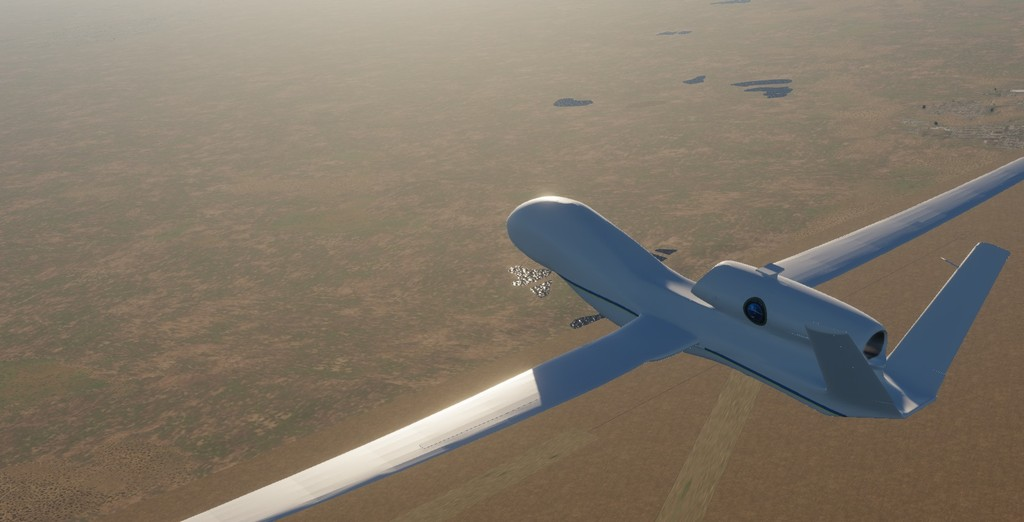
\includegraphics[width=\columnwidth]{aircraft.jpg}
\caption{The model in FlightGear, in its own livery. The 3-D model is NASA's, cut and rescaled (section~\ref{sec:fg}).}\label{fig:aircraft}
\end{figure}

\section{Reference data}\label{sec:ref}
When sources disagree the model follows the highest-ranked: a flight record of this aircraft, then a flight test of the type, then a tunnel test, then
another model, then handbook estimates. It is never tuned towards two sources at once, and a fit is made to one set of data and named
(section~\ref{sec:fits}). Table~\ref{tab:sources} lists the sources.

\begin{table}[t]
\centering\small
\caption{Sources and what they contribute.}\label{tab:sources}
\begin{tabularx}{\columnwidth}{@{}>{\raggedright\arraybackslash}p{2.5cm}X@{}}
\toprule
Source & Content used \\
\midrule
ATTREX records~\cite{attrex} & 26 flights of N872NA, 1 and 20\,Hz: attitude, angle of attack, Mach, pressure, winds, position; two landings to the rollout \\
Pastor et al.~\cite{pastor} & climb times and cruise-climb heights of two 2010 flights; take-off times \\
NASA briefings~\cite{ov,ops,upd} & dimensions, weights, ``flat rated at 7500\,lb'', endurance ``31+ hours'', how it is operated \\
NASA 3-D model, side view~\cite{glb} & planform shape, widths; lengths and heights \\
Jane's, quoted in~\cite{uthm} & wing area, span, length \\
TM~102840~\cite{lrn} & the LRN~1015 section and its tunnel test \\
Eaton and Woolf~\cite{sfte} & Block~20 flight test: lift-curve slopes, how the type flies, centre of gravity \\
ICAO databank~\cite{icao} & the AE~3007 variants at sea level: thrust, fuel flow, pressure and bypass ratio \\
Ghazi~\cite{ghazi} & the Citation~X's AE~3007C1 at maximum climb, 1500 and 45\,000\,ft \\
Rolls-Royce~\cite{rr}, EASA~\cite{easa} & engine layout, weight, speeds, fan diameter \\
Accident report~\cite{aib} & four navigators and their selection; the 2017 loss \\
Hobbs and Lyall~\cite{hl} & what a remote pilot station must show and control \\
\bottomrule
\end{tabularx}
\end{table}

The flight records have no weight, fuel, engine or control-surface channel. Weights are therefore the take-off weight, which is assumed (NASA's
25\,600\,lb for Pastor's flights, full tanks for ATTREX), less the model's own fuel flow along the measured flight. The days were not standard and the
model's atmosphere is.

\section{The model}\label{sec:model}
\subsection{Implementation}
One generator writes the JSBSim files from data files: the aerodynamic tables, the engine as system channels, the fuel system, the wing's bending, the
gear, and the flight laws, run at 120\,Hz. No Nasal is in the flight model. A harness drives the same files from Python to trim,
to find modes and to fly the checks.

\subsection{Geometry and mass}
NASA's 3-D model is an artist's model and not to scale: scaled to the published span its fuselage is 29\,\% too long, scaled to the length its span is
22\,\% short. No single scale brings it inside the limits set beforehand, so it gives shapes only. Positions along the length and heights come from NASA's
side-view drawing scaled by the published length; the wing's span stations from the 3-D model scaled by the published span; and the chords are scaled
so that the straight-tapered wing has the published 540\,ft$^2$ (figure~\ref{fig:geometry}). The wing so built is 6.83\,ft at the centreline and
2.47\,ft at the tip, swept 6.2$^\circ$ at the quarter chord; the V-tail's panels stand at 50$^\circ$ (published, and $50.8\pm0.5^\circ$ in two head-on photographs; the 3-D model's raw slope gave $47.1^\circ$ and was not used) and are 11.7\,ft long. Their lateral position and the gear's track are not the 3-D model's, which is not isotropic: two photographs of RQ-4As, a head-on view scaled by the tyre, a person and the aircraft's height and NASA's picture of N871 and N872 on the ramp fitted with one camera model, agree on a main-gear track of 10.8\,ft (11.2$\pm$0.5 and 10.1$\pm$0.7) and tail tips 10.2\,ft from the centreline (10.7$\pm$0.5 and 10.06$\pm$0.2), against 13.7 and 8.8\,ft before; the roots, at 2.7\,ft, follow from the tip, the rise and the angle. The section is the LRN~1015 \cite{lrn}.

\begin{figure*}[t]
\centering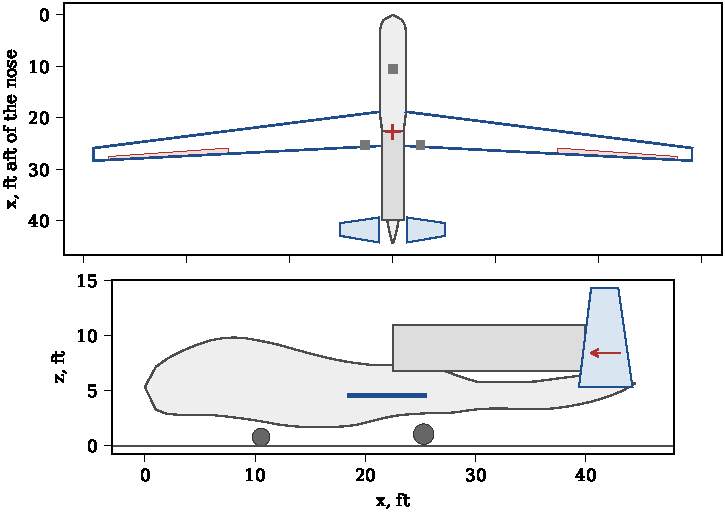
\includegraphics[width=0.86\textwidth]{geometry.pdf}
\caption{The geometry the flight model is built on. Ailerons (shaded) and the tail surfaces are estimates from photographs; the cross marks the centre
of gravity, the arrow the thrust line.}\label{fig:geometry}
\end{figure*}

Four weights are published: gross 26\,750\,lb, empty, fuel 15\,300\,lb and the engine's. The rest of the mass table is an estimate, and the centre
of gravity is a choice: 22\,\% of the mean chord, about 8\,\% ahead of the model's own neutral point. The fuel layout is the author's, six tanks drawn
down in proportion so that the centre of gravity stays put. The wing holds less than half the fuel. As the wing tanks empty the roll and yaw
inertias fall by almost three quarters.

\subsection{Aerodynamics}
The wing is 80 strips on a lifting line. Each strip takes lift, drag and moment from the section's table at its own angle of attack and Reynolds number
and the flight Mach number, and the trailing vortices of all strips give each its downwash. The V-tail's strips sit in the wing's downwash and sidewash;
fuselage and nacelle add friction drag and slender-body moments. The section data is NeuralFoil's \cite{nf}, with its compressibility correction. The
result is sampled into tables over angle of attack and Mach number, each Mach number at the height where the aircraft flies it. Ground effect is the
strip model's own vortices mirrored in the ground. A second build takes its tables from AeroSandbox's build-up method \cite{asb} on the same geometry;
it stood in for the CFD that does not exist (section~\ref{sec:aero}).

\subsection{Engine}
No map of the AE~3007H is public. The model is a two-spool, separate-exhaust cycle by the textbook analysis \cite{matt}, with fixed component
efficiencies and both turbines choked, and it treats the AE~3007 family as one piece of hardware run at different ratings. Its reference point is the
databank's row for the highest-rated variant, the A2 at 9494\,lbf, which is also Rolls-Royce's figure for the H. Maximum thrust is the lowest of three
limits: the flat rating, a turbine entry temperature, and the fan's corrected speed. Fuel flow is the cycle's above 60\,\% thrust and follows the shape
of the databank's points below 30\,\%. Thrust acts along the nacelle, 3.1\,ft above the centre of gravity. The spool is the fan's speed as a state: its share of the maximum here, thrust going
with the square of it, follows what the throttle asks at a rate that is limited and with a first-order lag (section~\ref{sec:engine}).

\subsection{Wing bending}
No stiffness, deflection or frequency of the wing is public. The bending is an estimate with a switch: a cantilever sized by strength (spar caps at a
strain of 0.0012 at 1\,$g$ and full weight), which gives a tip deflection of 4.3\,ft at full weight and 2.6\,ft at the cruise, and a first
frequency of 1.0 to 1.9\,Hz as the wing tanks empty. One mode is carried, driven by the lift and the load factor. Its use is twofold: the animation, and
the dihedral it gives, which slows the spiral by half and halves the Dutch roll's damping of the bare airframe.

\subsection{Gear, spoilers and the ground}
Three legs, the mains 10.8\,ft apart (two photographs), with estimated springs, nose-wheel steering, wheel brakes, and spoilers. The flight records show that the approach is flown on spoilers: at
4.5$^\circ$ of angle of attack the clean wing would carry a lift coefficient near 1.0 where the aircraft has 0.645, and its 4.45$^\circ$ glide needs a
lift-to-drag ratio of 13 where the clean aircraft has 28.

\subsection{Named fits}\label{sec:fits}
Fits are named, and a fitted figure does not count as a pass of what it was fitted to.
\begin{itemize}
\item \emph{Wing chords}: scaled to the published area.
\item \emph{The cycle's reference point}: fan pressure ratio, turbine temperature and efficiencies, to the A2's databank row.
\item \emph{The fan-speed limit}: to one number, the C1's thrust at 45\,000\,ft \cite{ghazi}; then raised 1\,\% with the drag increment.
\item \emph{An installation factor on fuel flow}, 6.2\,\% at 1500\,ft and 10.1\,\% from 45\,000\,ft: the Citation~X's installed engine against the
bare cycle. It is used unchanged, though the Global Hawk's installation is not the Citation~X's.
\item \emph{A drag increment}, 0.00308 (0.00355 before the tail's and the gear's lateral positions were measured; 0.00564, then 0.00586, before the CFD's wave drag went into the section data), and the 1\,\% on the fan-speed limit: to the measured climb above 40\,000\,ft and four cruise-climb heights
together. It adds 11\,\% to the model's own drag at cruise (0.0285 at Mach~0.6 and a lift coefficient of 0.96).
\item \emph{The wing's incidence}, 2.0$^\circ$: to the level of the ATTREX lift curve.
\item \emph{The spoilers' lift and drag}: to the 2013 approach's speed, glide and angle of attack at idle.
\item \emph{The rollout's deceleration}, 0.235\,$g$: the 2013 landing's.
\end{itemize}
Choices, not fits: the centre of gravity, the tail's incidence of $-3^\circ$ (ruddervators near neutral in cruise; two side photographs of RQ-4s read $-3.8\pm2^\circ$ and $-2.7\pm1.5^\circ$, checks that do not fit it), the control surfaces' sizes and
travel, the actuators, the structural limits of the hand-flown mode. They are assumptions and are listed in the data file's notes.

\subsection{Flight laws}\label{sec:lawsdesc}
The real laws are not public. These are built to behave as the sources say the aircraft does: in the climb the throttle is at maximum and the elevator
holds a scheduled airspeed \cite{pastor}; the ruddervators together are the elevator and against each other the rudder \cite{sfte}; turns are flown
at about 15$^\circ$ of bank at height and 21$^\circ$ low down. Inner loops hold pitch attitude, bank and zero sideslip with rate damping, gains following
dynamic pressure. Outer modes hold speed by the elevator or height with speed by thrust, a heading or a leg, and on the ground the nose wheel
follows the leg. The pitch command is a state that moves towards what the mode asks and is pulled down while the angle of attack is over a limit or the
speed under a floor. Approaches are flown as the records show: idle thrust, the elevator on the speed for a lift coefficient of 0.645, and the spoilers
holding a 4.45$^\circ$ glide path from a mid setting.

Above the laws a mission manager hands them the next leg, target and mode ten times a second and does nothing else. It exists twice, line for line: in
Python for the checks, and in FlightGear's scripting language for flight. Four navigators are modelled, each the true attitude plus an error a test
can set, with a vote: the middle value of three or four, and of two the one nearer a reference that no navigator supplies (the bank the turn rate
implies). Without an uplink for 30\,s the aircraft leaves its plan for the contingency route the plan carries; without the engine it glides to the
runway with the most height to spare and lands there.

A hand-flown mode is a simulator's addition, with two laws: one in which the stick asks for pitch rate and bank through the same protections, and one
direct. The real aircraft has neither.

\subsection{Ground station and FlightGear}\label{sec:fg}
The station is a page in a browser that talks to FlightGear's own web server: a map with the plan, the lost-link route and what is being flown; a flight
display; ranked alerts; commands that are shown before they are sent and count only when the aircraft answers; a plan editor with a forecast of time,
fuel, height and the landing's roll from a table sampled from the flight model; several stations with one in control and a handover; a link delay. In
FlightGear the aircraft carries NASA's 3-D model, rescaled to the published span, length and height, with its control surfaces cut out and a gear
that folds; a head-up display over the nose camera's picture; a belly camera that locks on a point or an object; and sounds synthesised from the engine's
and the airframe's physics \cite{pww}.

\section{Method}\label{sec:method}
The work went in phases, each with limits written before its first result. A limit is not moved afterwards and a miss stays printed until its cause is
fixed. One script runs every check on the model as committed and keeps the logs; another reads the logs into this report's tables and counts, and stops
on a miss that has no recorded cause. Table~\ref{tab:checks} gives the counts by what a check is held to.

\begin{table}[t]
\centering\small
\caption{All checks, pass/\textbf{miss}, by what they are held to: F a flight record of this aircraft, P a published figure or test, M another model or
another aircraft's data, D a design requirement of the author's, G generated (the model against the numbers it was generated from).}\label{tab:checks}
\begin{tabularx}{\columnwidth}{@{}>{\raggedright\arraybackslash}Xrrrrr@{}}
\toprule
 & F & P & M & D & G \\
\midrule
Engine &  & 8/\textbf{1} & 2/\textbf{2} &  &  \\
Engine against pyCycle &  &  & 12/\textbf{5} &  &  \\
Geometry and mass &  & 1/\textbf{8} &  &  & 3 \\
JSBSim model as generated &  &  &  & 8/\textbf{2} & 27/\textbf{1} \\
Section data and lift curve & 3 & 8/\textbf{1} &  &  &  \\
Climb, cruise-climb, endurance & 10 & 1 &  &  &  \\
Gear and ground & 7 &  &  & 5 &  \\
Wing bending &  &  &  &  & 4 \\
Flight laws &  &  &  & 44 &  \\
Landings and a whole mission & 8 &  &  & 10 &  \\
Navigators, lost link, engine out &  &  &  & 11 &  \\
Flown by hand &  &  &  & 26 &  \\
Station: link and commands &  &  &  & 13 &  \\
Station: alerts &  &  &  & 11 &  \\
Station: forecast &  &  &  & 4 &  \\
Station: several stations &  &  &  & 8 &  \\
Station: traffic and demo &  &  &  & 3 &  \\
FlightGear: starts &  &  &  & 5 &  \\
FlightGear: flown through the link &  &  &  & 10 &  \\
FlightGear: head-up display &  &  &  & 9 &  \\
FlightGear: belly camera &  &  &  & 5 &  \\
\midrule
All & 28 & 18/\textbf{10} & 14/\textbf{7} & 172/\textbf{2} & 34/\textbf{1} \\
\bottomrule
\end{tabularx}

\end{table}

The table is the measure of what this report can claim. \NFpass{} checks are held to flight records of the aircraft, and \Nfitted{} of those were
made after a fit to the same record. \NDpass{} are the laws and the software against requirements the author wrote for them: they show that the
design does what was asked of it and say nothing about the real aircraft. \Nreported{} further results are reported without a limit. The station's
own logic has \Nstationtests{} test files beside these, all passing.

The programme, run by run:
\begin{itemize}
\item \emph{the engine}: the cycle at the databank's conditions for the C1 and the A2, at Ghazi's two climb points, and at the H's altitude limit; the
same engine built in NASA's pyCycle \cite{pyc} with generic component maps, at the same points;
\item \emph{the section}: the section table at the tunnel's Mach and Reynolds numbers, compared at equal lift coefficient between 0.4 and 1.0, as the
tunnel report itself compares, because it calls its angles of attack uncertain by up to 3$^\circ$;
\item \emph{the mission}: the model trimmed at maximum thrust at each height and weight on Pastor's speed schedule, the flight-path angle giving the
climb rate (less the part that goes into airspeed rising with height) and the fuel flow taking the weight down, from 25\,600\,lb to 5\,\% of the fuel;
\item \emph{the lift curve}: level trims at the measured segments' mean Mach number and height over their range of weights, against the slope fitted
within flights, each flight with its own level, because the take-off weights are not known;
\item \emph{take-off and landing}: from rest at 25\,600\,lb at Edwards' height; the two recorded landings from 5\,nmi out at the weights the fuel
model gives for them, 20\,800 and 17\,100\,lb;
\item \emph{the laws}: steps, holds and a heading change at the cruise (Mach 0.6, 60\,000\,ft, 15\,000\,lb), a climb point (150\,KCAS, 10\,000\,ft, full
weight) and in the approach configuration, with the bending on and off; every gain doubled and halved; the climb from 10\,000 to 55\,000\,ft hands off;
\item \emph{a mission}: from a stand to a stand, taxi, take-off, three legs at 20\,000\,ft, landing, taxi in, nobody touching it;
\item \emph{failures}: a navigator's roll drifting 30$^\circ$ with two and with four in use; the uplink cut; the engine stopped 30 and 100\,nmi out;
\item \emph{by hand}: full stick held each way for 30\,s in the protected law, a simple pilot flying a task with the stick delayed, a dive in the direct law;
\item \emph{the station}: a scenario flown through its protocol against the flight model behind a stand-in for FlightGear's web server;
\item \emph{FlightGear}: the aircraft started on a runway and in the air, a flight by command alone through the link to a landing, the head-up
display read off screenshots, the camera held on a point and on a moving object.
\end{itemize}

\section{Results}\label{sec:results}
\subsection{The engine, on the Citation~X's variant first}\label{sec:engine}
\begin{figure*}[t]
\centering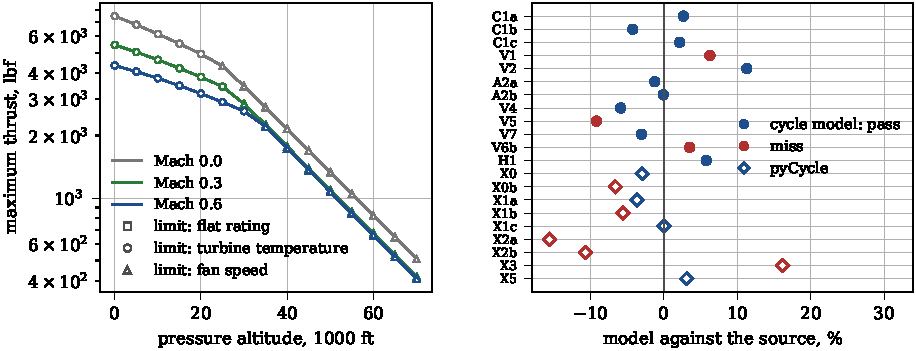
\includegraphics[width=\textwidth]{engine.pdf}
\caption{Left: maximum thrust as modelled, standard atmosphere, with the limit that sets it. Right: the engine checks, the cycle model and the pyCycle
build against the databank (C, A), Ghazi's table (V, X2, X3) and Rolls-Royce's pressure ratio (H1, X5).}\label{fig:engine}
\end{figure*}
Throttled back to the C1's rating, the cycle fitted to the A2 gives the C1's databank fuel flow within 2.7\,\%, its pressure ratio within 4.2\,\% and
its bypass ratio within 2.1\,\%, nothing of the C1 having been used (figure~\ref{fig:engine}). At 85\,\% thrust it burns 6.3\,\% more than the C1,
outside the 5\,\% limit, and 1.2\,\% less than the A2: the family's members differ by that much at one thrust, and the H's place among them is not known.
At maximum climb the bare cycle's specific fuel consumption is 5.9\,\% under the Citation~X's at 1500\,ft and 9.2\,\% under at 45\,000\,ft, the second
outside its 8\,\% limit; pyCycle's bare engine is 10.6\,\% under at the same point. Two bare models agreeing on that is the ground for reading the
difference as installation, which the installation factor then carries. At its altitude limit the cycle reaches a pressure ratio of 24.3 against
Rolls-Royce's 23.

Above 45\,000\,ft there is nothing to check the engine against. The two models, each with its fan-speed limit fitted to the same one number, agree
within 0.7\,\% on thrust and 1.4\,\% on fuel from 50\,000 to 65\,000\,ft; but in constant air temperature any cycle at a fixed corrected speed scales
its thrust with pressure, so this is weaker evidence than it looks. Neither has the loss of efficiency at low Reynolds number.

\emph{Power taken off the engine.} The Air Force's flight test names the power extracted for the payload as one of the conditions of the endurance
\cite{sfte}, and the cycle model had no term for it. It has one now: power taken off the high-pressure spool comes out of that spool's work balance, so
the compressor's pressure ratio and the core's flow fall at the same turbine temperature. The flight model has it as an input,
\texttt{engine/extra-power-kw}, above what the installation factor already holds (the Citation~X's own generators and bleed), zero at the start, so that
nothing else changes. At 60\,000\,ft and the cruise thrust, 20\,kW costs 2.5\,\% in fuel flow at 500\,lbf (a lift-to-drag ratio of 30 at 15\,000\,lb), 2.1\,\% at the flight model's cruise trim, and the
maximum thrust falls 0.5\,\%; at 10\,000\,ft the fuel changes by under 1\,\%. The fuel burned for it carries the power at a thermal efficiency of 0.47, inside
the 0.2 to 0.6 that any core must have. No data holds the size of the effect to anything: the ATTREX records carry no engine data, so this is a capability, not
a result. It does bound a suspect: 20 and 40\,kW cut the endurance, in the model as it was before the CFD's wave drag, from 34.7\,h to 34.0 and 33.2, so payload power does not explain NASA's 31.

\emph{The spool.} Thrust followed a single lag of 2\,s, a class estimate. A recording of a Citation~X taking off (outside, at Portland; audio only) has the
fan's blade-passing tone and its second harmonic clean enough to track: from about 1\,700\,Hz it rises to a plateau of 2\,885\,Hz in about two seconds, the
aircraft nearly standing (Doppler under 3\,\%). Normalised, the fan speed goes from 0.60 to 0.90 of its final value in 1.24\,s and to 0.98 in 1.76\,s; the
first part is a rate limit (a first-order lag alone would do 0.6 to 0.8 in 0.34\,s, it took 0.66), the last a lag. The fan's speed is now a state that
rises at 0.23 of its value a second at most and with a lag of 0.38\,s, fitted to the track by least squares (rms 0.019); the model reproduces 0.6 to 0.9 in
1.31\,s and to 0.98 in 1.92\,s (limits 20\,\%, after the fit). The old lag gave 5.55\,s for the last, and 5.67 for thrust from 15 to 95\,\%, over the 5\,s
that the certification rule for transport engines allows (recalled, not checked), where the new gives 3.7. What the recording does not show is the rise from
idle (the tone is under the noise below 0.6 of the final speed): half the measured rate there, and the same going down, are estimates, and the engine is a
Citation~X's AE~3007C1, not the H. In flight the plain take-off's 130\,KIAS time went from 32.8 to 34.2\,s (12.5 to 8.8\,\% under Pastor's) and the laws' from
32.4 to 32.7; the estimate of the low-range rate is most of that, so it is not claimed as a result. The fan's rpm for the sound and the 3-D model is the state itself.

\subsection{The section against the tunnel}\label{sec:section}
\begin{figure*}[t]
\centering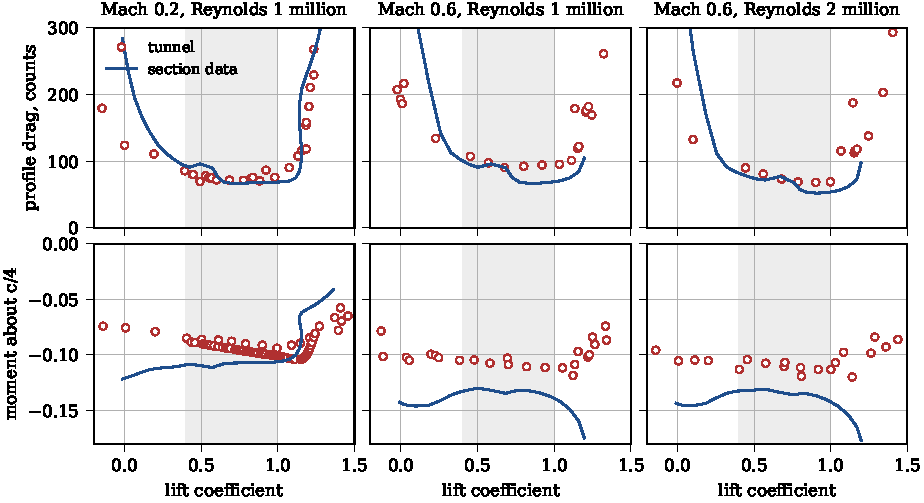
\includegraphics[width=\textwidth]{section.pdf}
\caption{The wing section's data against NASA's tunnel test of the LRN~1015 \cite{lrn}, digitised from its figure~24. The band is the range compared.}\label{fig:section}
\end{figure*}
Between lift coefficients of 0.4 and 1.0 the section data's drag is 6\,\% over the tunnel's at Mach~0.2 and 13 to 14\,\% under it at Mach~0.6, inside
the 15\,\% limit but one-sided where the wing cruises (figure~\ref{fig:section}). Wing profile drag is about 45\,\% of the aircraft's drag at cruise, so
this alone makes the uncalibrated model's lift-to-drag ratio some 6\,\% too good.

The moment was the section's weak point. As the data first came from NeuralFoil it was 0.013 more nose-down than the tunnel's at Mach~0.2 and 0.023 to
0.025 at Mach~0.6, the last outside the limit of 0.02, because it grew 24\,\% from Mach~0.2 to 0.6 (the Prandtl--Glauert factor alone is 22\,\%) where the tunnel's grew 15.5\,\%. XFOIL \cite{xfoil}, built for this report and run on the same section with its
Kármán--Tsien correction, gives 19\,\% and a moment of $-0.105$ at Mach~0.2 where NeuralFoil gives $-0.108$ and the tunnel $-0.0945$: the two solvers agree
with each other and lie 0.010 to 0.013 more nose-down than the tunnel at low speed, which no compressibility correction touches. XFOIL cannot be run
where it matters: past the first sonic point at Mach~0.6 it stops converging, and gives six and eight points only. The growth of the moment was
therefore fitted, with one parameter, to the tunnel's: the wing's moment goes as $\beta^{-0.65}$ instead of $\beta^{-1}$, $\beta=\sqrt{1-M^2}$ (the
exponent is that which gives the tunnel's 1.155 between the two Mach numbers, \texttt{strips.CM\_MACH\_K}). The two Mach~0.6 cases now miss by 0.015
and 0.013, inside the limit, and Mach~0.2 is as it was. The same change made the bare airframe's speed mode at the cruise stable, which was not
its aim: each table of the aerodynamic model, held at its Mach~0.45 values above that Mach number, was tried, and only the moment's growth with Mach
number moved the unstable root (a real root doubling in 10\,s; \texttt{fdm/section\_study.py}). The drag increment was refitted afterwards, from 0.00564
to 0.00586, because the time from 10\,000 to 55\,000\,ft had moved to 6.1\,\% against a limit of 5. It was fitted again, to 0.00355, when the CFD's wave drag went into the section data (below), and to 0.00308 when the tail's lateral position was measured.

Maximum lift stops at 1.20 at Mach~0.6, where the data puts a shock stall; the tunnel reached 1.31 and 1.42, the second a miss. XFOIL cannot say who is
right, so a transonic solver was built for this report: SU2 on a wall-resolved mesh of 40\,000 cells, Spalart--Allmaras, fully turbulent, 42 cases. The rule fixed
beforehand was to trust it for the stall only if its moment at the tunnel's lifts came within 0.02 of the tunnel's at both Mach~0.6 cases and its maximum lift
within 10\,\% at the first. It did not: its moment is 0.028 and 0.026 more nose-down than the tunnel's, as XFOIL's and NeuralFoil's are, so nothing in the tables
changed. It does not agree with the model's stall either: its maximum lift at Mach~0.6 is 1.37 and 1.40, 5\,\% over and 2\,\% under the tunnel's and 13 and 16\,\% over
the model's, while its fall to Mach~0.65 (22\,\%) is about the model's (18\,\%). The tunnel and the solver agree that the model stalls early at Mach~0.6, on the side
that is safe for the laws; a fit of the model's stall to the tunnel's two figures is what the evidence now supports, and was left undone because the rule said so.
The solver also puts the growth of the moment from Mach~0.2 to 0.6 at 1.105, the tunnel's 1.139: below the 1.237 of the original tables, and so on the side of the
exponent fitted above.

\emph{What was then done with the solver.} Its rise of section drag with Mach number at equal lift, from Mach~0.45 to 0.55, 0.6, 0.65 and 0.7 at a Reynolds number of 1.5 million (95 cases in all), was added to the wing's drag table as a difference within the solver, because its absolute drag is about twice the tunnel's: the correction is the solver's rise less the table's own. The test written for it (the correction smooth in Mach number) failed as written, because the table's own rise at Mach~0.7 is erratic, and the rule for which cases to trust, by density residual, was found to drop well-converged cases and keep worse ones, and was replaced by the lift spread alone; both changes are recorded in the plan, with the first rule's result beside them. The solver's own rise does not fall with Mach number at any of 47 supported points. At lift coefficients 0.4, 0.6, 0.8 and 0.95 the correction is +10, +12, +13 and +22 counts of section drag at Mach~0.6, and +21, +43, +73 and +170 at 0.65. The best lift-to-drag ratio in the tables falls from 37.2 to 34.1 at Mach~0.6 and from 31.1 to 24.3 at 0.65, and the drag increment, fitted again, from 0.00586 to 0.00355 (0.00308 after the lateral dimensions, below). Taking each change out in turn showed what it did to the checks: the trimmed lift-curve slope at Mach~0.6 left its limit (+15.6\,\%) because the heaviest three of six weights no longer trim at full throttle at 57\,000\,ft, and the climb to 55\,000\,ft is 9\,\% short. A fit of the model's stall to the tunnel's two maxima, with the solver's shape, was made and met the maximum-lift check, and was withdrawn: in its blend back to the table's own stall after the solver's last angle the lift fell 0.26 to 0.37 per degree where the solver's steepest fall is 0.13, which its own limits ruled out. The maximum-lift miss at Mach~0.6 stays.

\subsection{The two aerodynamic models}\label{sec:aero}
At Mach~0.6 and 2.5$^\circ$ the strips and AeroSandbox's build-up give lift-curve slopes of 0.134 and 0.132 per degree, neutral points at 29.8 and
32.5\,\% of the mean chord, roll damping within 10\,\% and aileron power 20\,\% apart; both reach a lift-to-drag ratio of 34 to 36 untrimmed. They
differ by a factor of two to three in pitch and yaw damping, between the reference's own two methods as much as between it and the strips, which the
laws' gain margins have to cover. No limit was set on these: the spread is each quantity's uncertainty. Against the Air Force's flight test of the
longer-winged Block~20 \cite{sfte}, whose figures give slopes but no absolute values, the strips' untrimmed lift-curve slope is within 3\,\% at Mach
0.575 and 0.60 and 6 to 16\,\% steep below Mach~0.55.

That paper refers the aircraft's performance to a centre of gravity at 31\,\% of the mean chord. Both models put the neutral point at 30 to 33\,\%.
Either the real neutral point is further aft than both say, or the real aircraft flies with little static margin and leaves stability to its
control system. The model keeps 22\,\%, with a static margin of 8.5\,\% of the chord at the cruise trim (60\,000\,ft, Mach~0.60, 15\,000\,lb) and 4.6 and 4.3\,\% at 50\,000\,ft (Mach~0.58, 20\,000\,lb) and 55\,000\,ft
(Mach~0.61, 17\,000\,lb) (finite differences of the strip model over $\pm0.5^\circ$, ruddervators at their trims; the step matters near the section's moment kink at 3.5 to 4$^\circ$: 1$^\circ$ gives 7.1, 5.9 and 5.8\,\%). Setting the V-tail at its published 50$^\circ$, from the 3-D model's 47$^\circ$, took about 1.9\,\% of the chord from each (from 9.8, 5.6 and 5.3\,\%) and the horizontal tail volume from 0.277 to 0.236, and the measured lateral position of its tips gave 0.6 to 0.8 back; the Phase~1 aim of 5\,\% is then not met at the two heavier conditions, which is reported and not refitted. At 31\,\% the margin would be $-0.5$\,\% at the cruise and $-4$ to $-5$\,\% at the other two: so a centre of gravity at 31\,\% in this model is unstable, and it cannot be moved there without a reason the data does not
give. It is the largest open question of the aerodynamic model; the paper may also mean only the point its moments are referred to.

The ATTREX records at 20\,Hz carry something no earlier data did here: in 260 steady, level stretches above 50\,000\,ft of 16 flights, the spectra of pitch rate
(the derivative of the attitude), angle of attack and vertical acceleration all have a peak, three times over the median or more in every one: the aircraft's
short period, excited by turbulence. Its median is 0.293\,Hz (middle half 0.244 to 0.352) with a damping of about 0.15; the 2013 flights give 0.24 to 0.26\,Hz
and the 2014--2015 flights 0.33 to 0.40, a step that a change of the flight control or the configuration could explain and nothing here does. The model's bare
airframe has 0.185 to 0.230\,Hz at the same conditions and its laws, in MIL-F-8785C turbulence, 0.303 to 0.322 (with the V-tail at 50$^\circ$ and its tips at their measured place; 0.234 to 0.279 and 0.303 to 0.322 before). By the reading fixed beforehand (the peak
within 30\,\% of the model's closed loop) the margin is supported and the 22\,\% stays. What the data cannot do is tell the real flight control from the bare
airframe: the frequency goes with the dynamic pressure to the power 1.05, where the model's bare airframe goes to 0.43 and its closed loop to nearly nothing.
They do say that the real pitch stiffness is at least the model's, so that a near-neutral aircraft is not what flew (unless the flight control supplied it all).

\subsection{Climb, cruise-climb and the lift curve in flight}\label{sec:calib}
\begin{figure*}[t]
\centering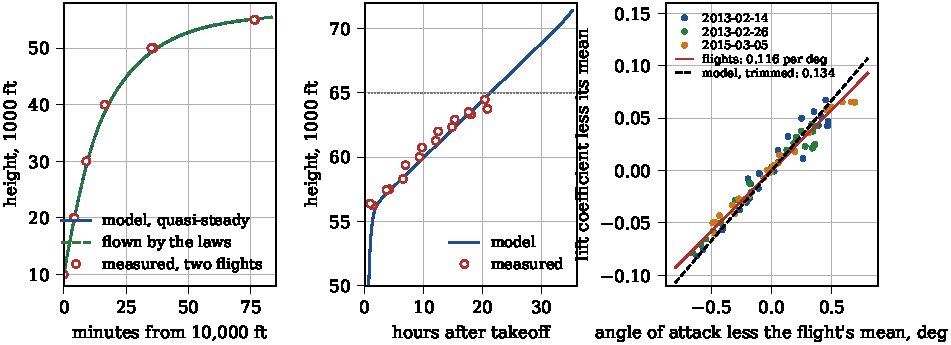
\includegraphics[width=\textwidth]{calibration.pdf}
\caption{Against the flights. Left: the climb from 10\,000\,ft, the quasi-steady mission and the same climb flown in time by the laws, against Pastor's
two flights \cite{pastor}. Middle: the cruise-climb. Right: lift against angle of attack in the steady segments of three ATTREX flights at Mach 0.59
to 0.62, each flight about its own mean, with the slope fitted to them and the model's trimmed slope.}\label{fig:calib}
\end{figure*}
With the engine as section~\ref{sec:engine} left it, the flat rating read as a cap of 7500\,lbf, the model climbed at 3560\,ft/min at 10\,000\,ft where
Pastor measured about 2450. The thrust the measured climb needs at 15\,000\,ft, with the model's drag, is about 4200\,lbf. The turbine temperature at
which the cycle gives 4200\,lbf there is 1254\,K, and 1254\,K is the temperature at which it gives 7500\,lbf at rest at sea level. The rating is
therefore read as one limit on turbine temperature, held at every height. Nothing was fitted for it, and the climb rates from 10\,000 to 40\,000\,ft
then came out 4.3, 5.9 and 10.5\,\% under the measured ones, inside their 15\,\% limits (figure~\ref{fig:calib}); with the drag increment
of the final fit below, 1.8, 2.5 and 4.8\,\%.

Above 40\,000\,ft two numbers were fitted together, a drag increment and a factor on the fan-speed limit, to the climb rates there and four cruise-climb
heights. They sit in a shallow valley: fan-speed factors from 1.00 to 1.02 with increments from 0.0019 to 0.0043 fit almost equally. Thrust and drag
cannot be told apart with this data. After the fit the time from 10\,000 to 55\,000\,ft is 4182\,s against 4596 (9.0\,\% short: a miss, the limit being 5), and the model follows the measured
cruise-climb within 890\,ft for 20 hours at a lift coefficient of 0.96 and a lift-to-drag ratio of 30. Left alone it goes on climbing as it empties, past the
65\,000\,ft NASA quotes as the maximum, which the laws hold as a limit. Flown in time by the laws, the same climb takes 4077\,s.

\emph{Endurance} from 14\,500\,lb of fuel to 5\,\% left, with NASA's 65\,000\,ft maximum height held once it is reached (the schedule's Mach number
kept, the engine throttling back), is 34.9\,h; NASA says ``31+''. The window set beforehand was 29 to 35\,h, and it is met, by 0.1\,h. That window is a sanity check and not a measurement:
``31+'' is a capability claim; the one official record for the RQ-4A is 30\,h 24\,min (2001, a record flight), and later blocks have flown 33 hours (2008)
and, in a squadron's unregistered record, 34.8, with reserves and payloads nobody states. A model fitted to the 30.4 would be fitted to a flight
whose conditions are unknown, so it was not: where the physics gives more, the model says more. The figure says only what the earlier miss was: the quasi-steady mission, with nothing to stop it, climbed on as it emptied to 71\,450\,ft with the tanks nearly dry and
reached 35.1\,h (35.4 before the section's moment was corrected), a height NASA does not give for any flight. That figure is kept in the log as a reported
line, and the ceiling is reached 21.8\,h after take-off. Nothing was changed in the model for this. A fuel-flow
factor was allowed for and not used, and stays unused: a fan-speed factor of 1.04 with a drag increment of 0.0068 would give 31.3\,h at 1.4 times the misfit to
the climb, and a change of 10\,\% in fuel flow, well beyond the engine's stated uncertainty of 6\,\%, would be needed with the fit as it is, to match a
figure that is not a measurement of this aircraft.

\begin{figure}[t]
\centering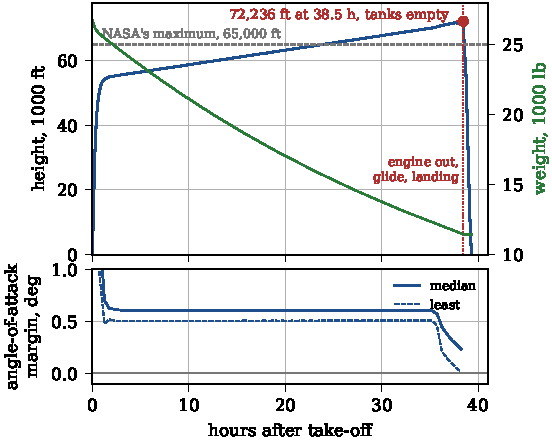
\includegraphics[width=\columnwidth]{record.pdf}
\caption{The highest the model flies: full tanks to empty, cruise-climbing at Mach 0.6 with the 65\,000\,ft limit lifted, then the engine-out glide and landing. Below, the angle-of-attack margin, its median and its least value in each half hour (a turn of the racetrack uses 0.5$^\circ$ of it by design).}\label{fig:record}
\end{figure}
\emph{The highest the model flies, tanks run dry.} The same aircraft flown through its own laws and mission manager, offline, with nothing held at 65\,000\,ft: it takes off at 26\,750\,lb
with all 15\,300\,lb of fuel that the model's tanks hold, cruise-climbs at maximum thrust on the schedule's Mach number (0.6 above FL550) round a racetrack with 150\,nmi sides, so that the field is always within glide
range, and when the tanks are empty (under 2\,lb) the engine is failed, the way the fuel running out would stop it, and the aircraft's own engine-out logic glides it to the field and lands it. The
laws' and the manager's 65\,000\,ft limits are lifted for this run only. \emph{The model reaches 72\,236\,ft, 38.5\,h after take-off, with the tanks empty (11\,452\,lb) at Mach 0.600; the flight is 39.3\,h in all} (figure~\ref{fig:record}).
The height is 56\,988\,ft at 6\,h, 62\,374 at 18, 65\,043 at 24 (NASA's maximum passed), 67\,762 at 30 and 70\,707 at 36\,h; with 2\,000\,lb of fuel left 68\,260\,ft, with 1\,000\,lb 69\,912, with 500\,lb 71\,156 and with 100\,lb 72\,038.
The climb rate is 8 to 15\,ft/min throughout and 25 near 36\,h. The angle-of-attack margin is 0.61$^\circ$ up to 35\,h, 0.25$^\circ$ at 38\,h and 0.19$^\circ$ in the last minutes: the aircraft is at the coffin corner when
the fuel runs out, and a few hundred feet more are all that is left. The engine fails 98\,nmi from the field; the glide takes 51\,min and the landing is 4.5\,ft off the runway line, the rollout 4.5\,ft at most. Above 65\,000\,ft
this is the model extrapolated, not the aircraft measured: the engine data go to 70\,000\,ft and Mach 0.7, the aerodynamic data are sampled at 60\,000\,ft for Mach 0.6 and the laws' tables go to 65\,000\,ft and are held at their last value above it.
The quasi-steady mission above reached 71\,450\,ft with its tanks nearly dry, 790\,ft lower: it burns 14\,500\,lb, this flight 15\,300. Neither is a flight to set a number beside: NASA gives 65\,000\,ft as the maximum and no flight to more.

\emph{Lift curve.} The records' angle of attack is pitch attitude less flight-path angle within 0.2$^\circ$ all flight. In the steady segments of three
flights at Mach 0.59 to 0.62 the trimmed slope is 0.116 per degree; the model's, from trims over the same weights, is 0.123, 5.6\,\% over. One flight
at Mach 0.50 to 0.54 gives 0.130 against the model's 0.134. The flights' levels differ by 0.09 in lift coefficient, which is 10\,\% of weight or
0.7$^\circ$ of incidence: the wing's incidence was set to their mean, and only the slope is a prediction. In 409 turns of 90\,s or more the measured
bank is that which speed times turn rate gives within 0.06$^\circ$ on average.

\subsection{Take-off and landing}\label{sec:ground}
\begin{figure*}[t]
\centering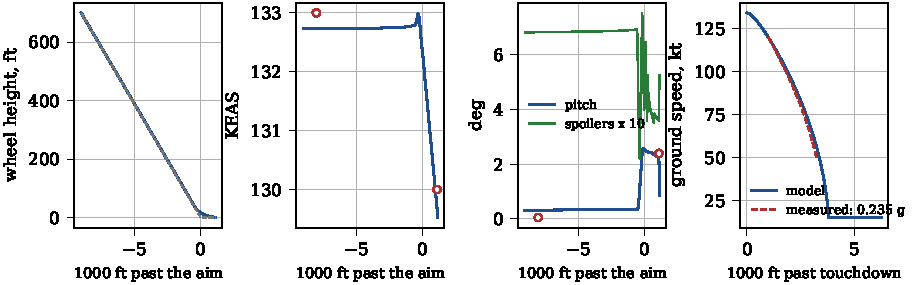
\includegraphics[width=\textwidth]{landing.pdf}
\caption{The 2013 landing flown by the laws at 20\,800\,lb. Circles: the record's approach and touchdown values. Right: the rollout against the record's
steady 0.235\,$g$.}\label{fig:landing}
\end{figure*}
From brake release the model reaches 130\,KIAS in 32.8\,s where Pastor's flights took 37 and 38, lifts off at 134\,KEAS where 19 records begin at 121
to 139, climbs at 2770\,ft/min half a minute later, inside the records' 2250 to 3650, and takes 54\,s from 2500 to 5000\,ft against 59 to 63. It is
12\,\% quick on the runway and 11\,\% in the first climb, both inside their limits and both the same way: a little too much thrust less drag low down,
at an assumed weight. Flown by the laws, which rotate at 120\,KIAS to 6.5$^\circ$ (numbers of the design, set against the records' ranges, not
fitted to one flight; the first rotation speed was Pastor's 130\,KIAS milestone, which is no rotation speed), the aircraft reaches 130\,KIAS in 32.4\,s,
13.6\,\% before Pastor's, and lifts off at 138\,KEAS and 6.9$^\circ$, inside the records' 121 to 139\,KEAS and 4.5 to 7$^\circ$ at the top of both.

The two recorded approaches are at 133 and 120\,KEAS. Their ratio is that of the square roots of the two landing weights the fuel model gives within
half a percent, so the approach is flown at one lift coefficient, and the laws' rule for it picks 132.8 and 120.4\,KEAS. With the spoilers fitted to the
2013 approach, the 2014 approach trims at idle thrust at an angle of attack of 4.79$^\circ$ against the measured 4.29$^\circ$. Flown by the laws
(figure~\ref{fig:landing}) the touchdowns come at 129.4 and 117.7\,KEAS and a pitch attitude of 2.3$^\circ$, against 130 and 122\,KEAS and 2.4 and
2.3$^\circ$, sinking 0.66 and 0.69\,m/s where the aircraft touched at 0.66 and 0.75, and 960 to 1060\,ft past the aiming point. The rollout holds
0.22\,$g$. These touchdowns are not predictions: the flare law's four numbers (its height, 45\,ft; its target attitude; the sink it asks for, 1.6\,m/s;
the spoiler gain) were chosen with the two records' touchdown in view. The first flare the laws had touched down at 1.1\,m/s, which looked like a fault
in the model and was one in the law; of the candidates tried, this is the one that stayed within five knots of the records' speeds as well as the sink.
The step of the integration is not what decides them: take-off and landing figures at 240, 480 and 960\,Hz differ from those at 120 by 1\,kt and 0.5$^\circ$
at most (\texttt{fdm/rate\_study.py}), and a frame costs 16\,$\mu$s.

\subsection{The laws}\label{sec:laws}
\begin{figure*}[t]
\centering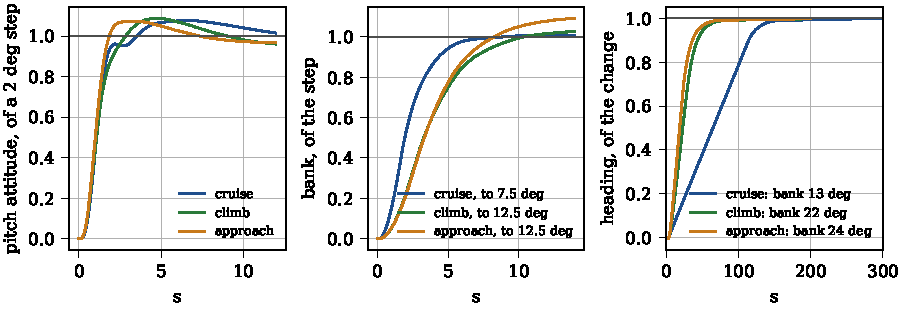
\includegraphics[width=\textwidth]{laws.pdf}
\caption{The laws' responses at the three conditions: a pitch step, a bank step to half the bank limit, a heading change of 90$^\circ$.}\label{fig:laws}
\end{figure*}
A pitch step of 2$^\circ$ overshoots 8 to 9\,\% and settles in 1.9\,s; a bank step settles in 4 to 7\,s; a heading change of 90$^\circ$ ends within
0.2$^\circ$ at 13$^\circ$ of bank at the cruise and 22 to 24$^\circ$ lower (figure~\ref{fig:laws}). Height is held within 0.5\,ft for 300\,s at the
cruise and the climb point. A sideslip of 2$^\circ$ is under 0.2$^\circ$ after three periods of the bare airframe's Dutch roll. The bare airframe had
an unstable aperiodic speed mode at the cruise, doubling in 10\,s, where lift and moment change with Mach number near 0.6; its cause was the
section's moment growing with Mach number faster than the tunnel's (section~\ref{sec:section}), and with that corrected the airframe's long mode is a
phugoid of 176\,s with a damping ratio of 0.06. Corrected, the cruise trim needs 1.7$^\circ$ of ruddervator where it needed 0.7$^\circ$, which showed
a fault in the checks: the trim had left its ruddervator command in the stick property, 0.087 of full travel where the protected law's dead band is
0.05, and the cruise's hands-off test read it as a push on the stick. The checks now start with the stick at neutral. Every gain doubled and every gain halved, the loops stay stable; phase margin was not measured. All 44 checks pass, and all are the
laws against their own limits: nothing of the real aircraft's response to a control is public to hold them to.

\subsection{A mission, hands off}
\begin{figure*}[t]
\centering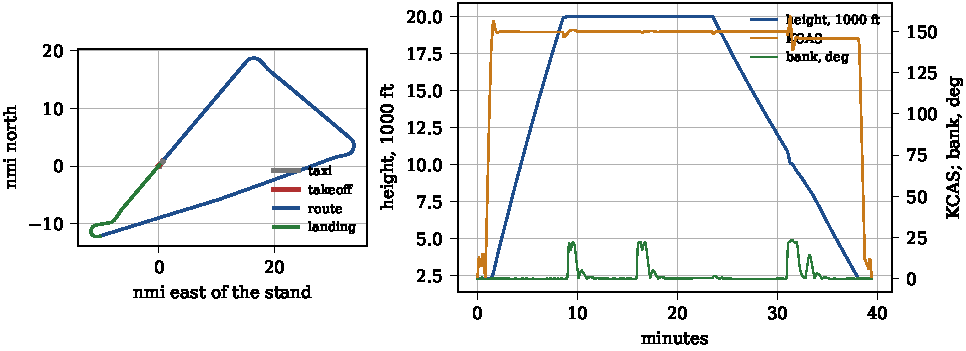
\includegraphics[width=\textwidth]{flight.pdf}
\caption{A mission from a stand to a stand under the laws and the mission manager, at 25\,600\,lb from a field at 2300\,ft.}\label{fig:flight}
\end{figure*}
The mission of figure~\ref{fig:flight} takes 39 minutes and 558\,lb of fuel and ends 11\,ft from its last point. Taxi stays within 9\,ft of the path
in the corners; the take-off reaches 130\,KIAS in 32.7\,s and lifts off at 137\,KEAS and 6.9$^\circ$, inside the records' 121 to 139\,KEAS and 4.5 to 7$^\circ$, and 30 to 40\,s
later flies at 149\,KEAS, 10.9$^\circ$ and 2\,790\,ft/min, inside the records' 147 to 151, 10 to 14 and 2\,250 to 3\,650 (the speed was 153 before the speed mode's integral
gain was raised); heights are captured within 149\,ft and held within 16; the cross-track error is under 0.25\,nmi for 95\,\% of the route, with up to
2.4\,nmi in its two sharp turns, which the laws round; the landing holds the glide path within 0.8\,ft and touches down at 0.64\,m/s.

\subsection{Days that are not standard, wind and turbulence}\label{sec:offdesign}
Nothing public holds any of this to a figure, so the limits are the design's own, written before the runs (phase~11 in the logs). \emph{Days.} The engine tables
run from $-40$ to $+40$\,K of temperature offset. On days of $-20$, $+15$ and $+30$\,K the laws hold height within 0.5\,ft and speed within 0.02\,kt hands off at the
high, climb and low conditions (at $+30$\,K the high one has no level trim: the thrust is not there); the maximum thrust at 20\,000\,ft falls 0.55\,\% a kelvin
from $-20$\,K to standard and 0.87 from standard to $+15$\,K; the 2013 landing is as on a standard day at $-20$ and $+30$\,K. One limit missed, and it was wrong: that
the time from 10\,000 to 55\,000\,ft grows with the temperature. Above 22\,000\,ft the schedule is in Mach number (rising to 0.60 at 55\,000\,ft), so the climb rate goes with the true airspeed,
which falls in the cold, and thrust and drag both go with pressure: the cold day is 3\,\% slower (3\,479 against 3\,369\,s); the hot days lose their ceilings
(about 54\,000\,ft at $+15$ and 50\,000 at $+30$\,K). A first version of this check compared geometric heights, where 55\,000\,ft on a $-20$\,K day is 59\,500 of
pressure, and took the physics for a fault. \emph{Turbulence and wind.} MIL-F-8785C turbulence as JSBSim has it gives nothing at altitude at severity~1, so severity 5
at 60\,000\,ft (2.0\,m/s rms) and 3 at 20\,000 (1.1) were used, one deterministic draw and not statistics. The laws hold height within 75 and 69\,ft and bank within
0.9 and 1.8$^\circ$ with no structural flag, and the load factor stays between 0.71 and 1.25\,g; the airspeed varies by 11 to 12\,kt against a limit of 5, which is a
miss that no loop could avoid, since the gust along the heading itself varies by 15 to 25\,kt. The whole mission in a 25\,kt wind from the runway heading with light
turbulence is flown in 40 minutes, with 94\,\% of the route inside 0.25\,nmi (95 was asked; the phase~7b rule of 80 passes) and a stop at 0.9\,kt where 0.5 was asked, two more
misses on the margin. The 2013 landing in a 10\,kt crosswind with light turbulence is down 8\,ft from the centreline at 0.31\,m/s; at 20\,kt 7\,ft and 0.5; in severe turbulence
(severity 5, 4\,m/s at the field) 50\,ft and 1.3\,m/s. Two faults of mine in these checks are worth the record: JSBSim's wind is reset to nothing by every initial-conditions
call, so the first mission and landings were flown without the wind; and a trim made with turbulence on fails, and the landings that followed it came down at 6 to 7\,m/s, an
artefact that nearly led to a change of the flare for the wrong reason. The change that stayed: the flare starts at a time to touchdown when the sink is more than a
downdraft's (2.6\,s at the sink beyond 4\,ft/s above the approach's own), which at severity 5 turned a 3.3\,m/s touchdown 460\,ft short into 1.3\,m/s and changes nothing in calm air.

\subsection{Gusts and the landing: the stabilisation and the speed addition}\label{sec:gusts}
The landing law holds the glide path with the spoilers and the speed with the pitch, and the throttle is at idle from the glide to the touchdown. The question was what a gust does
to it and whether two additions help: a \emph{stabilisation} (the switch \texttt{ap/gust-sys}; only in the landing, in the air, under 500\,ft: the speed law may not take the nose under
$-1^\circ$ in the glide; the throttle follows the speed lost beyond 4\,kt, with its own rate limits and idle in the flare; the pitch goes up with the sink that the spoilers, at their
floor, cannot take) and an \emph{addition} to the approach speed (\texttt{ap/approach-add-kt} by hand, or \texttt{ap/approach-add-auto}: the aircraft's own pick from the spread of the wind about its
10\,s mean and the share of the wind across the final). Both switches were 0 when these flights were flown, and with them at 0 the flights are those of the aircraft without them (99 flights flown
again: no difference); the aircraft now ships with both at 1 (section~\ref{sec:rules}). A gust alert, raised whether the stabilisation is on or not, tells the station (\emph{caution}: 8\,kt of speed lost or 8\,ft/s more sink than the path asks, held 4\,s).
\emph{Method.} The flights are the bench's (\texttt{fdm/gustbench.py}): the landing task alone from 5\,nmi out on the glide, calm trim, wind written into the model every frame in the runway's axes. Gusts
are discrete 1-cosine gusts (along, vertical, across; sizes and heights as the table says) and the bench's own MIL-F-8785C low-altitude Dryden turbulence at a wind at 20\,ft of 30 to 60\,kt, alone and
with that wind blowing steadily at 45$^\circ$ to the runway; JSBSim's own turbulence is not used, because in this harness it is the same at every height and for every wind at 20\,ft. The four arms (neither;
the speed alone; the stabilisation alone; both) are flown on the same cases, so every comparison is paired. The system and the pick's tables were designed and fitted on other flights (the discrete gusts of
the design sweeps, and turbulence seeds 1 to 16); the flights below are a test set written before the fit was frozen and flown once: 216 discrete gusts the design never saw (three weights, other sizes, heights and
rise times) and 48 turbulence sequences a weather (seeds 101 to 148). A \emph{hard landing} is a sink over 2\,m/s, the structural flag, or no touchdown (2\,m/s is a convention of mine); an \emph{event} is a flight
in which the angle-of-attack protection acted (the margin under 0) below 500\,ft. The contrasts are paired differences with 95\,\% bootstrap intervals (10\,000 resamples of the cases) and, for the hard landings,
the exact McNemar test on the pairs that differ, at a level of 0.017 (three contrasts on this measure). The numbers are this model's, in the bench's gusts: discrete gusts are stress cases and a share of them is not a rate in service,
the turbulence is not the real air's, and there are no real gust data in the sources to hold any of it to.

\begin{table*}[t]\centering\footnotesize
\begin{tabular}{@{}l r r r r r r r r@{}}
\toprule
Arm & Flights & Hard & Sink, mean (m/s) & Sink, 95\,\% & Events & Line, 95\,\% (ft) & Nose, 95\,\% ($^\circ$) & Landing (ft) \\
\midrule
\multicolumn{9}{@{}l}{\textbf{discrete: a lost or gained headwind (96 cases)}} \\
\quad neither & 96 & 73 & 6.56 & 14.02 & 2 & 3.1 & 0.2 & 4\,120 \\
\quad speed alone & 96 & 73 & 6.56 & 14.02 & 2 & 3.1 & 0.2 & 4\,120 \\
\quad stabilisation alone & 96 & 42 & 3.39 & 10.99 & 3 & 3.1 & 0.2 & 4\,827 \\
\quad both & 96 & 42 & 3.39 & 10.99 & 3 & 3.1 & 0.2 & 4\,827 \\
\quad fixed +10\,kt alone & 96 & 78 & 7.53 & 14.85 & 0 & 3.1 & 0.2 & 4\,511 \\
\quad fixed +10\,kt with the system & 96 & 45 & 3.67 & 12.51 & 0 & 3.0 & 0.2 & 5\,317 \\
\midrule
\multicolumn{9}{@{}l}{\textbf{discrete: a downdraught (72 cases)}} \\
\quad neither & 72 & 46 & 3.50 & 8.42 & 2 & 3.1 & 0.1 & 4\,031 \\
\quad speed alone & 72 & 46 & 3.50 & 8.42 & 2 & 3.1 & 0.1 & 4\,031 \\
\quad stabilisation alone & 72 & 31 & 2.39 & 6.48 & 6 & 3.1 & 0.1 & 4\,172 \\
\quad both & 72 & 31 & 2.39 & 6.48 & 6 & 3.1 & 0.1 & 4\,172 \\
\quad fixed +10\,kt alone & 72 & 38 & 3.18 & 8.44 & 0 & 3.1 & 0.1 & 4\,669 \\
\quad fixed +10\,kt with the system & 72 & 29 & 2.13 & 7.12 & 0 & 3.1 & 0.1 & 4\,796 \\
\midrule
\multicolumn{9}{@{}l}{\textbf{discrete: a gust across (48 cases)}} \\
\quad neither & 48 & 0 & 0.69 & 0.73 & 0 & 12.6 & 2.7 & 4\,684 \\
\quad speed alone & 48 & 0 & 0.69 & 0.73 & 0 & 12.6 & 2.7 & 4\,684 \\
\quad stabilisation alone & 48 & 0 & 0.69 & 0.73 & 0 & 12.6 & 2.7 & 4\,683 \\
\quad both & 48 & 0 & 0.69 & 0.73 & 0 & 12.6 & 2.7 & 4\,683 \\
\quad fixed +10\,kt alone & 48 & 0 & 0.58 & 0.64 & 0 & 7.1 & 1.5 & 5\,306 \\
\quad fixed +10\,kt with the system & 48 & 0 & 0.58 & 0.62 & 0 & 8.0 & 1.9 & 5\,261 \\
\midrule
\multicolumn{9}{@{}l}{\textbf{turbulence, a wind at 20 ft of 30 kt (48 sequences)}} \\
\quad neither & 48 & 1 & 0.93 & 1.68 & 48 & 8.4 & 2.1 & 4\,993 \\
\quad speed alone & 48 & 3 & 1.25 & 2.16 & 38 & 7.4 & 2.5 & 5\,423 \\
\quad stabilisation alone & 48 & 1 & 0.97 & 1.70 & 48 & 8.4 & 2.2 & 5\,013 \\
\quad both & 48 & 0 & 1.02 & 1.56 & 39 & 9.9 & 2.9 & 5\,507 \\
\midrule
\multicolumn{9}{@{}l}{\textbf{turbulence, a wind at 20 ft of 40 kt (48 sequences)}} \\
\quad neither & 48 & 6 & 1.29 & 2.33 & 48 & 11.4 & 3.3 & 5\,076 \\
\quad speed alone & 48 & 10 & 1.29 & 2.27 & 48 & 9.9 & 2.9 & 5\,107 \\
\quad stabilisation alone & 48 & 8 & 1.29 & 2.77 & 48 & 11.7 & 3.1 & 5\,161 \\
\quad both & 48 & 4 & 1.19 & 2.27 & 48 & 10.2 & 3.4 & 5\,233 \\
\midrule
\multicolumn{9}{@{}l}{\textbf{turbulence, a wind at 20 ft of 50 kt (48 sequences)}} \\
\quad neither & 48 & 18 & 1.66 & 3.08 & 48 & 14.7 & 5.3 & 5\,269 \\
\quad speed alone & 48 & 17 & 1.64 & 2.89 & 48 & 18.7 & 3.5 & 5\,316 \\
\quad stabilisation alone & 48 & 19 & 1.70 & 3.28 & 48 & 14.9 & 4.1 & 5\,463 \\
\quad both & 48 & 20 & 1.70 & 3.05 & 48 & 19.6 & 3.2 & 5\,534 \\
\midrule
\multicolumn{9}{@{}l}{\textbf{turbulence, a wind at 20 ft of 60 kt (48 sequences)}} \\
\quad neither & 48 & 34 & 2.12 & 3.34 & 47 & 26.8 & 4.2 & 5\,510 \\
\quad speed alone & 48 & 32 & 2.29 & 4.84 & 48 & 22.5 & 5.6 & 5\,475 \\
\quad stabilisation alone & 48 & 34 & 2.02 & 3.64 & 48 & 25.6 & 4.8 & 5\,850 \\
\quad both & 48 & 36 & 2.00 & 4.25 & 48 & 23.2 & 4.1 & 5\,594 \\
\midrule
\multicolumn{9}{@{}l}{\textbf{turbulence with a steady wind at 45 deg, a wind at 20 ft of 30 kt (48 sequences)}} \\
\quad neither & 48 & 2 & 1.09 & 1.77 & 47 & 10.1 & 7.3 & 3\,658 \\
\quad speed alone & 48 & 2 & 0.98 & 1.77 & 48 & 13.7 & 6.9 & 3\,662 \\
\quad stabilisation alone & 48 & 0 & 0.97 & 1.67 & 47 & 9.2 & 6.1 & 3\,815 \\
\quad both & 48 & 2 & 0.95 & 1.69 & 47 & 12.5 & 5.9 & 3\,843 \\
\midrule
\multicolumn{9}{@{}l}{\textbf{turbulence with a steady wind at 45 deg, a wind at 20 ft of 40 kt (48 sequences)}} \\
\quad neither & 48 & 7 & 1.32 & 2.37 & 48 & 25.2 & 10.9 & 3\,170 \\
\quad speed alone & 48 & 10 & 1.40 & 2.51 & 48 & 22.6 & 10.7 & 3\,109 \\
\quad stabilisation alone & 48 & 7 & 1.28 & 2.36 & 48 & 21.9 & 9.6 & 3\,495 \\
\quad both & 48 & 8 & 1.30 & 2.33 & 48 & 23.6 & 9.2 & 3\,460 \\
\midrule
\multicolumn{9}{@{}l}{\textbf{turbulence with a steady wind at 45 deg, a wind at 20 ft of 50 kt (48 sequences)}} \\
\quad neither & 48 & 19 & 1.98 & 5.19 & 48 & 41.0 & 17.3 & 2\,346 \\
\quad speed alone & 48 & 18 & 2.41 & 8.76 & 48 & 35.5 & 18.3 & 2\,295 \\
\quad stabilisation alone & 48 & 11 & 1.46 & 2.45 & 48 & 41.3 & 13.2 & 3\,001 \\
\quad both & 48 & 16 & 1.47 & 2.43 & 48 & 38.0 & 13.8 & 2\,995 \\
\bottomrule
\end{tabular}

\caption{The four arms on the test set. Hard: flights that landed hard; events: flights in which the angle-of-attack protection acted below 500\,ft; line and nose: the distance off the centreline and the
nose's heading error at the first wheel (95th percentiles); landing: the distance from the aiming point to the end of the rollout (mean). The fixed +10\,kt arms are the same with the addition set by hand.}\label{tab:gust4}
\end{table*}
\begin{table*}[t]\centering\footnotesize
\begin{tabular}{@{}l l r r r r l l l@{}}
\toprule
Contrast & Hard & Only first & Only second & $p$ & & $\Delta$ sink (m/s) & $\Delta$ line (ft) & $\Delta$ landing (ft) \\
\midrule
\multicolumn{9}{@{}l}{\textbf{discrete: a lost or gained headwind (96 cases)}} \\
\quad speed against neither & 73 against 73 & 0 & 0 & 1.000 & & +0.00 [+0.00, +0.00] & +0.0 [+0.0, +0.0] & +0 [+0, +0] \\
\quad stabilisation against neither & 42 against 73 & 0 & 31 & $<$0.001 & & -3.17 [-3.97, -2.40] & -0.1 [-0.2, -0.0] & +706 [+520, +894] \\
\quad both against neither & 42 against 73 & 0 & 31 & $<$0.001 & & -3.17 [-3.98, -2.41] & -0.1 [-0.2, -0.0] & +706 [+526, +894] \\
\quad fixed +10\,kt against neither & 78 against 73 & 6 & 1 & 0.125 & & +0.97 [+0.66, +1.31] & -0.2 [-0.3, -0.1] & +391 [+296, +476] \\
\quad fixed +10\,kt with the system against stabilisation & 45 against 42 & 3 & 0 & 0.250 & & +0.28 [+0.08, +0.51] & -0.1 [-0.2, -0.1] & +490 [+416, +558] \\
\midrule
\multicolumn{9}{@{}l}{\textbf{discrete: a downdraught (72 cases)}} \\
\quad speed against neither & 46 against 46 & 0 & 0 & 1.000 & & +0.00 [+0.00, +0.00] & +0.0 [+0.0, +0.0] & +0 [+0, +0] \\
\quad stabilisation against neither & 31 against 46 & 0 & 15 & $<$0.001 & & -1.12 [-1.47, -0.80] & -0.0 [-0.0, +0.0] & +141 [+81, +213] \\
\quad both against neither & 31 against 46 & 0 & 15 & $<$0.001 & & -1.12 [-1.48, -0.79] & -0.0 [-0.0, +0.0] & +141 [+82, +210] \\
\quad fixed +10\,kt against neither & 38 against 46 & 1 & 9 & 0.021 & & -0.33 [-0.51, -0.14] & -0.2 [-0.3, -0.1] & +638 [+593, +682] \\
\quad fixed +10\,kt with the system against stabilisation & 29 against 31 & 2 & 4 & 0.688 & & -0.26 [-0.42, -0.09] & -0.1 [-0.2, -0.1] & +624 [+588, +661] \\
\midrule
\multicolumn{9}{@{}l}{\textbf{discrete: a gust across (48 cases)}} \\
\quad speed against neither & 0 against 0 & 0 & 0 & 1.000 & & +0.00 [+0.00, +0.00] & +0.0 [+0.0, +0.0] & +0 [+0, +0] \\
\quad stabilisation against neither & 0 against 0 & 0 & 0 & 1.000 & & +0.00 [+0.00, +0.00] & -0.0 [-0.0, +0.0] & -1 [-1, -0] \\
\quad both against neither & 0 against 0 & 0 & 0 & 1.000 & & +0.00 [+0.00, +0.00] & -0.0 [-0.0, +0.0] & -1 [-1, -0] \\
\quad fixed +10\,kt against neither & 0 against 0 & 0 & 0 & 1.000 & & -0.11 [-0.11, -0.11] & -2.3 [-3.3, -1.2] & +622 [+604, +640] \\
\quad fixed +10\,kt with the system against stabilisation & 0 against 0 & 0 & 0 & 1.000 & & -0.11 [-0.11, -0.10] & -1.9 [-2.9, -0.9] & +578 [+566, +590] \\
\midrule
\multicolumn{9}{@{}l}{\textbf{turbulence, a wind at 20 ft of 30 kt (48 sequences)}} \\
\quad speed against neither & 3 against 1 & 3 & 1 & 0.625 & & +0.32 [-0.02, +0.76] & -0.2 [-0.8, +0.5] & +430 [+295, +562] \\
\quad stabilisation against neither & 1 against 1 & 0 & 0 & 1.000 & & +0.04 [-0.07, +0.15] & +0.1 [-0.1, +0.4] & +20 [-9, +49] \\
\quad both against neither & 0 against 1 & 0 & 1 & 1.000 & & +0.10 [-0.09, +0.29] & +0.1 [-0.6, +0.9] & +515 [+410, +622] \\
\midrule
\multicolumn{9}{@{}l}{\textbf{turbulence, a wind at 20 ft of 40 kt (48 sequences)}} \\
\quad speed against neither & 10 against 6 & 6 & 2 & 0.289 & & +0.00 [-0.19, +0.20] & -0.5 [-1.4, +0.4] & +31 [-74, +138] \\
\quad stabilisation against neither & 8 against 6 & 5 & 3 & 0.727 & & +0.00 [-0.18, +0.19] & +0.5 [-0.0, +1.1] & +85 [+25, +147] \\
\quad both against neither & 4 against 6 & 2 & 4 & 0.688 & & -0.10 [-0.25, +0.05] & +0.1 [-0.8, +1.0] & +156 [+59, +253] \\
\midrule
\multicolumn{9}{@{}l}{\textbf{turbulence, a wind at 20 ft of 50 kt (48 sequences)}} \\
\quad speed against neither & 17 against 18 & 7 & 8 & 1.000 & & -0.02 [-0.28, +0.23] & +0.8 [-0.2, +1.8] & +47 [-54, +149] \\
\quad stabilisation against neither & 19 against 18 & 2 & 1 & 1.000 & & +0.04 [-0.22, +0.28] & -0.1 [-0.8, +0.6] & +194 [+96, +327] \\
\quad both against neither & 20 against 18 & 10 & 8 & 0.815 & & +0.04 [-0.27, +0.33] & +1.3 [+0.0, +2.6] & +265 [+115, +451] \\
\midrule
\multicolumn{9}{@{}l}{\textbf{turbulence, a wind at 20 ft of 60 kt (48 sequences)}} \\
\quad speed against neither & 32 against 34 & 3 & 5 & 0.727 & & +0.17 [-0.12, +0.48] & -0.2 [-2.0, +1.5] & -36 [-162, +98] \\
\quad stabilisation against neither & 34 against 34 & 6 & 6 & 1.000 & & -0.10 [-0.54, +0.22] & +0.1 [-1.1, +1.3] & +340 [+158, +567] \\
\quad both against neither & 36 against 34 & 8 & 6 & 0.791 & & -0.12 [-0.61, +0.30] & +0.0 [-1.8, +1.8] & +84 [-130, +315] \\
\midrule
\multicolumn{9}{@{}l}{\textbf{turbulence with a steady wind at 45 deg, a wind at 20 ft of 30 kt (48 sequences)}} \\
\quad speed against neither & 2 against 2 & 1 & 1 & 1.000 & & -0.12 [-0.30, +0.05] & +1.0 [-0.1, +2.2] & +4 [-63, +69] \\
\quad stabilisation against neither & 0 against 2 & 0 & 2 & 0.500 & & -0.12 [-0.42, +0.10] & -0.4 [-1.3, +0.4] & +157 [+70, +256] \\
\quad both against neither & 2 against 2 & 2 & 2 & 1.000 & & -0.15 [-0.44, +0.09] & +0.6 [-0.3, +1.6] & +185 [+88, +293] \\
\midrule
\multicolumn{9}{@{}l}{\textbf{turbulence with a steady wind at 45 deg, a wind at 20 ft of 40 kt (48 sequences)}} \\
\quad speed against neither & 10 against 7 & 6 & 3 & 0.508 & & +0.08 [-0.12, +0.30] & -1.5 [-3.8, +0.5] & -61 [-138, +17] \\
\quad stabilisation against neither & 7 against 7 & 3 & 3 & 1.000 & & -0.04 [-0.44, +0.25] & -1.3 [-2.8, +0.1] & +325 [+193, +470] \\
\quad both against neither & 8 against 7 & 5 & 4 & 1.000 & & -0.02 [-0.45, +0.28] & -2.2 [-4.4, +0.1] & +290 [+149, +457] \\
\midrule
\multicolumn{9}{@{}l}{\textbf{turbulence with a steady wind at 45 deg, a wind at 20 ft of 50 kt (48 sequences)}} \\
\quad speed against neither & 18 against 19 & 4 & 5 & 1.000 & & +0.43 [-0.06, +1.01] & +0.9 [-1.5, +3.5] & -51 [-153, +48] \\
\quad stabilisation against neither & 11 against 19 & 3 & 11 & 0.057 & & -0.52 [-0.99, -0.14] & -0.2 [-3.2, +2.9] & +655 [+401, +953] \\
\quad both against neither & 16 against 19 & 2 & 5 & 0.453 & & -0.51 [-0.95, -0.14] & +0.2 [-3.5, +3.8] & +649 [+402, +945] \\
\bottomrule
\end{tabular}

\caption{The contrasts, paired by case. Hard: the flights that landed hard in the first and in the second arm; only first and only second: the pairs in which only that arm's flight landed hard; $p$: the exact
McNemar test of those; the differences are the first arm less the second, means with 95\,\% bootstrap intervals.}\label{tab:gustc}
\end{table*}

\emph{Results.} The stabilisation lands softer in a lost headwind and in a downdraught: hard landings fell from 73 to 42 of 96 cases and from 46 to 31 of 72, with no case made worse ($p<0.001$ in each),
and the mean sink fell by 3.2\,m/s and 1.1\,m/s. It does nothing for a gust across the runway (the line and the nose are the same to a tenth) and \emph{nothing that can be told from chance in turbulence}: no
contrast on the hard landings in the seven turbulent weathers is under the level, the nearest being the stabilisation against neither at 50\,kt with the steady wind (19 to 11 of 48, $p=0.06$, the sink 0.5\,m/s lower)
and both against the speed alone at 40\,kt ($p=0.03$). The aircraft's own pick of the speed addition is nothing in calm air, so in the discrete gusts the speed arms are the plain ones; in turbulence it is 12\,kt in a wind at
20\,ft of about 30\,kt, where it takes the events from 48 to 38 of 48 for 430\,ft of landing and no gain in sink (3 hard landings against 1), and nothing above that. A fixed +10\,kt, which a rule of thumb would give, makes the
sink worse in a lost headwind (+1.0\,m/s) and a little better in a downdraught (hard landings 46 to 38, $p=0.02$, the sink 0.3\,m/s lower), for 400 to 640\,ft of landing, and adds nothing to the stabilisation ($p=0.25$ and 0.69);
across the runway it narrows the line (12.6 to 7.1\,ft). At a wind at 20\,ft of 50 and 60\,kt, 18 and 34 of 48 flights land hard in every arm: the landing law has no answer to turbulence of that strength, and this is open.
In FlightGear the same final with a 15\,kt loss of headwind at 99\,ft (full fuel, 26\,750\,lb) touched down at 9.35\,m/s and 9.1\,g with a structural alert without the stabilisation, and at 0.33\,m/s and 1.1\,g with it.
\emph{What it comes to.} The stabilisation is worth having for the shears and downdraughts and is not for turbulence; the speed addition has no demonstrated benefit in this model beyond the angle-of-attack margin in light turbulence,
and costs runway; the sections that follow put the addition beside the airliners' rules and say why both switches are now on. \emph{Two faults of mine.} The bench's turbulence was first 59\,\% as strong as its label (a unit error, and a check of it that used the same formula and so passed):
every result before the fix was thrown away and flown again, and the fit above was made on the corrected flights, which supported a much smaller pick than the first. And the first small comparison I made (15 to 9 of 20) rested on 20 cases of a
design grid; the table above has 96, 72 and 48.

\subsection{The airliners' rules of thumb, and the aircraft's own laws}\label{sec:rules}
The speed addition above is a rule of thumb, and airliners fly with two well-known ones. The question was whether either does for this aircraft what the stabilisation and the pick do.
\emph{The rules} are my readings of them: the Boeing one from memory and not checked against a manual, the Airbus one from the open-source A320-family aircraft for FlightGear (its \texttt{FMGC.nas}),
with the live headwind taken as a component, which that file does not do. Boeing's adds half the steady headwind component and the whole gust increment (twice the along-wind $\sigma$ of the turbulence at 30\,ft, the way a pilot
would work it from a reported mean wind and gust), limited to 5 to 20\,kt; Airbus's adds a third of the headwind component, 5 to 15\,kt, with or without the ground-speed minimum (the approach speed raised by how far
the live headwind exceeds the tower's). Each is flown alone and with the stabilisation, on the same cases as the arms above. \emph{The air} is now JSBSim's own MIL-F-8785C turbulence as FlightGear runs it, at the field's height,
with the rotation of the gusts across the wings that the bench's Dryden lacks (a bench without it did not reproduce the lateral wander of the FlightGear flights): 336 sequences (seven weathers at 20\,800\,lb, seeds 601 to 648) and
the two FlightGear weathers that went wrong in flight, 28\,kt abeam with turbulence and 36\,kt abeam with a shear to 85\,kt at 500\,ft (48 sequences each, 26\,750\,lb). The laws were frozen for these flights (version~2).
The first reading of the table showed Boeing equal to Airbus in every turbulence-only weather: the bench took the Boeing rule's gust increment from the old turbulence's name and got zero from the new one. It was fixed
and the Boeing arms were flown again; the first results are kept.

\begin{table*}[t]\centering\footnotesize
\begin{tabular}{@{}l r r r r r r@{}}
\toprule
Arm & Hard (flagged) & Events & Sink, mean (m/s) & Sink, 95\,\% & Line, 95\,\% (ft) & Landing (ft) \\
\midrule
\multicolumn{7}{@{}l}{\textbf{seven turbulence weathers pooled, 20\,800\,lb (336 sequences)}} \\
\quad no addition & 92 (8) & 336 & 1.68 & 3.86 & 27.5 & 3\,698 \\
\quad stabilisation alone & 80 (7) & 336 & 1.52 & 3.37 & 33.4 & 3\,896 \\
\quad own pick and stabilisation & 74 (7) & 336 & 1.50 & 3.46 & 32.2 & 3\,902 \\
\quad Boeing rule & 105 (36) & 144 & 2.10 & 7.15 & 41.8 & 4\,446 \\
\quad Boeing rule with the stabilisation & 82 (13) & 199 & 1.51 & 3.46 & 36.4 & 4\,804 \\
\quad Airbus rule & 88 (20) & 272 & 1.92 & 6.48 & 35.4 & 3\,975 \\
\quad Airbus rule with the stabilisation & 74 (4) & 279 & 1.50 & 3.50 & 36.2 & 4\,260 \\
\midrule
\multicolumn{7}{@{}l}{\textbf{28\,kt abeam with turbulence, 26\,750\,lb (48 sequences)}} \\
\quad no addition & 4 (1) & 48 & 1.26 & 2.47 & 31.9 & 4\,874 \\
\quad stabilisation alone & 5 (2) & 47 & 1.18 & 2.36 & 28.4 & 5\,016 \\
\quad own pick and stabilisation & 5 (2) & 48 & 1.17 & 2.40 & 34.5 & 5\,021 \\
\quad Boeing rule & 15 (9) & 11 & 1.83 & 7.84 & 42.6 & 5\,769 \\
\quad Boeing rule with the stabilisation & 9 (9) & 12 & 0.96 & 1.61 & 39.8 & 5\,913 \\
\quad Airbus rule & 11 (6) & 38 & 1.97 & 9.01 & 36.7 & 5\,010 \\
\quad Airbus rule with the stabilisation & 4 (3) & 37 & 1.17 & 1.94 & 39.1 & 5\,378 \\
\midrule
\multicolumn{7}{@{}l}{\textbf{36\,kt abeam with the shear to 85\,kt at 500\,ft, 26\,750\,lb (48 sequences)}} \\
\quad no addition & 47 (42) & 39 & 13.73 & 23.56 & 64.2 & 605 \\
\quad stabilisation alone & 30 (20) & 47 & 2.19 & 5.37 & 62.2 & 4\,187 \\
\quad own pick and stabilisation & 30 (19) & 47 & 2.10 & 3.96 & 58.0 & 4\,157 \\
\quad Boeing rule & 45 (43) & 4 & 14.32 & 23.41 & 98.9 & -224 \\
\quad Boeing rule with the stabilisation & 33 (31) & 20 & 2.84 & 11.07 & 99.3 & 4\,350 \\
\quad Airbus rule & 47 (45) & 30 & 15.38 & 23.65 & 71.5 & 23 \\
\quad Airbus rule with the stabilisation & 31 (23) & 44 & 2.87 & 8.63 & 97.9 & 4\,172 \\
\bottomrule
\end{tabular}

\caption{The airliners' rules against the aircraft's own laws (the pick and the stabilisation), in JSBSim's own turbulence. Hard: sink over 2\,m/s, the structural flag or no touchdown; events: flights in which the angle-of-attack
protection acted below 500\,ft (the margin under its limit below 0); line: the distance off the centreline at the first wheel (95th percentile); landing: the distance from the aiming point to the end of the rollout (mean).}\label{tab:rules}
\end{table*}
\begin{table*}[t]\centering\footnotesize
\resizebox{\textwidth}{!}{\begin{tabular}{@{}l l r r r l l@{}}
\toprule
Contrast & Hard & Only first & Only second & $p$ & $\Delta$ sink (m/s) & $\Delta$ landing (ft) \\
\midrule
\multicolumn{7}{@{}l}{\textbf{seven turbulence weathers pooled, 20\,800\,lb (336 sequences)}} \\
\quad own pick and stabilisation against no addition & 74 against 92 & 19 & 37 & 0.022 & -0.18 [-0.30, -0.06] & +204 [+163, +247] \\
\quad Boeing rule against no addition & 105 against 92 & 68 & 55 & 0.279 & +0.42 [+0.14, +0.70] & +747 [+646, +848] \\
\quad Airbus rule against no addition & 88 against 92 & 43 & 47 & 0.752 & +0.24 [+0.02, +0.48] & +277 [+211, +344] \\
\quad own pick and stabilisation against Boeing rule & 74 against 105 & 45 & 76 & 0.006 & -0.60 [-0.86, -0.35] & -544 [-645, -437] \\
\quad own pick and stabilisation against Airbus rule & 74 against 88 & 35 & 49 & 0.156 & -0.42 [-0.65, -0.21] & -73 [-141, -2] \\
\quad own pick and stabilisation against Boeing rule with the stabilisation & 74 against 82 & 43 & 51 & 0.470 & -0.01 [-0.16, +0.13] & -902 [-967, -840] \\
\quad own pick and stabilisation against Airbus rule with the stabilisation & 74 against 74 & 39 & 39 & 1.000 & -0.00 [-0.15, +0.14] & -358 [-412, -302] \\
\midrule
\multicolumn{7}{@{}l}{\textbf{28\,kt abeam with turbulence, 26\,750\,lb (48 sequences)}} \\
\quad Boeing rule against no addition & 15 against 4 & 14 & 3 & 0.013 & +0.57 [-0.08, +1.30] & +895 [+708, +1070] \\
\quad Airbus rule against no addition & 11 against 4 & 9 & 2 & 0.065 & +0.71 [+0.04, +1.52] & +136 [-31, +285] \\
\quad own pick and stabilisation against Boeing rule & 5 against 15 & 3 & 13 & 0.021 & -0.66 [-1.38, -0.02] & -748 [-933, -550] \\
\quad own pick and stabilisation against Airbus rule & 5 against 11 & 3 & 9 & 0.146 & -0.80 [-1.57, -0.15] & +11 [-156, +195] \\
\midrule
\multicolumn{7}{@{}l}{\textbf{36\,kt abeam with the shear to 85\,kt at 500\,ft, 26\,750\,lb (48 sequences)}} \\
\quad stabilisation against no addition & 30 against 47 & 1 & 18 & $<$0.001 & -11.53 [-13.06, -9.94] & +3582 [+3227, +3941] \\
\quad Boeing rule against no addition & 45 against 47 & 1 & 3 & 0.625 & +0.59 [-2.02, +3.13] & -829 [-1289, -368] \\
\quad Airbus rule against no addition & 47 against 47 & 1 & 1 & 1.000 & +1.65 [-0.34, +3.70] & -582 [-798, -377] \\
\quad own pick and stabilisation against Boeing rule & 30 against 45 & 2 & 17 & $<$0.001 & -12.21 [-14.15, -10.13] & +4381 [+3940, +4806] \\
\quad own pick and stabilisation against Airbus rule & 30 against 47 & 0 & 17 & $<$0.001 & -13.28 [-15.09, -11.30] & +4135 [+3752, +4532] \\
\bottomrule
\end{tabular}
}
\caption{The contrasts that carry the argument, paired by case; columns as table~\ref{tab:gustc}. Differences are the first arm less the second, means with 95\,\% bootstrap intervals.}\label{tab:rulesc}
\end{table*}

\emph{What the rules buy.} What they are made for: room before the stall. The angle-of-attack protection acts below 500\,ft in all 336 flights with no addition and with the aircraft's own, in 144 with Boeing's rule and in 272 with Airbus's
(199 and 279 with the stabilisation); the median room under its limit goes from $-1.9^\circ$ to $+0.2^\circ$ (Boeing) and $-1.0^\circ$ (Airbus), and the share of flights 2$^\circ$ or more over the limit from 42\,\% to 1 and 20\,\%.
\emph{What they cost.} Sink: Boeing's rule adds 0.42\,m/s on average [$+0.14$, $+0.70$] and Airbus's 0.24 [$+0.02$, $+0.48$], and the sink's 95th percentile goes from 3.9 to 7.2 and 6.5\,m/s; the landing is 277 (Airbus) to 748\,ft (Boeing)
longer; the hard landings are not fewer (105 and 88 against 92; $p=0.28$ and 0.75); and Boeing's rule crosses the assumed structural limits (2.5\,$g$ or 200\,KEAS in the air, a latched flag) in 36 flights and Airbus's in 20, against 8 with no addition. On top of the stabilisation they add nothing that can be seen in the sink (1.50, 1.51 and 1.50\,m/s) or in the hard landings (82 and 74 against 80),
for 364 to 908\,ft of landing. The two FlightGear weathers say the same. At 28\,kt abeam Boeing's rule lands 15 of 48 flights hard against 4 ($p=0.013$). In the shear no rule touches the 47 hard landings of 48 (45, 47 and 48: an addition of
5 to 16\,kt against a shear of 85\,kt), where the stabilisation takes them to 30 ($p<0.001$: 18 flights only without it, 1 only with).

\emph{What the aircraft's own laws do.} The stabilisation lands softer where this aircraft lands hard: in a lost headwind or a downdraught (hard landings 73 to 42 of 96 and 46 to 31 of 72, $p<0.001$ in each; flown again in JSBSim's own turbulence on the version~2 laws, 72 to 42 and 44 to 31), and in the
shear (47 to 30 of 48; the median sink from 13.9 to 1.8\,m/s). In turbulence the pooled count of the first run is 92 to 74 of 336 with the pick and the stabilisation ($-5.4$ points [$-9.7$, $-1.0$], $p=0.022$: above the level of 0.017 this report set for
itself, so suggestive and not shown) and the sink 0.18\,m/s lower [$-0.30$, $-0.06$]. (The replicate below finds less: 101 to 92, and nothing at the light weight.) It buys no margin: the protection acts in the same 336 flights, up to 6.1$^\circ$ over its limit against 4.9$^\circ$ with no addition. So the two kinds of law
protect against different things. The rules keep the angle of attack away from the lift break and pay in sink and runway; the stabilisation keeps the sink down at the touchdown and does nothing for the margin. For an aircraft with no one aboard a landing
protected at the price of the margin is a calculated risk that a design can take, and this model cannot say how large it is: its lift curve at approach Mach numbers is still rising at the last point of its table (12$^\circ$), so it has no stall to be near, and the
limit of 7$^\circ$ is the design's own number (the lift break less a margin). What can be said is the price of the margin: Airbus's rule with the stabilisation has the same 74 hard landings and 1.50\,m/s of sink as the aircraft's own pick, with 57 fewer flights over the
limit, for 358\,ft of runway.

\emph{The same flights again.} The arms the argument rests on were flown again on the laws as they now stand, with the stiffer roll loop of section~\ref{sec:tips}, at two other weights (12\,450 and 26\,750\,lb, 168 sequences each, the same seven weathers, seeds 801 to 824:
2\,016 flights, the laws frozen for the run, and the comparisons of the aircraft's own system with each rule written down as a prediction before the flights were looked at; tables~\ref{tab:rulesv3} and~\ref{tab:rulesv3c}).
\emph{Confirmed.} Against Boeing's rule alone the aircraft's own system has 92 hard landings against 157 ($p<0.001$), 0.66\,m/s less sink [$-0.99$, $-0.35$] and 368\,ft less landing, at both weights (59 against 76, $p=0.030$, at 12\,450\,lb; 33 against 81, $p<0.001$, at 26\,750\,lb); and the rules hold
more margin: the protection acts in 193 (Boeing) and 270 (Airbus) flights against 328 with the aircraft's own, and the median room under its limit is $-0.3^\circ$ and $-1.3^\circ$ against $-1.9^\circ$.
\emph{Half confirmed.} Against Airbus's rule alone the sink is lower (0.26\,m/s [$-0.48$, $-0.05$]) and the hard landings fewer, but not by a margin that can be told from chance (92 against 98, $p=0.54$; 74 against 88, $p=0.16$ in the first run).
\emph{Not as predicted.} With the stabilisation on, Boeing's rule is far worse than the aircraft's own system (148 hard landings against 92, $p<0.001$), where in the first run they were level (82 against 74, $p=0.47$). The extra hard landings are structural: the flag that marks a crossing of the assumed limits is raised in 97 flights with that arm
and 32 with the aircraft's own (102 and 27 for Boeing's rule alone and for no addition), against 13 and 7 at the one weight of the first run. Boeing's addition, 16\,kt on average here, makes the approach faster, and a gust loads the structure in proportion to the speed; the rule trades the stall limit for the structural one. Airbus's rule with the stabilisation is level
with the aircraft's own (95 hard landings against 92, $p=0.82$, the sink the same) and lands 326\,ft longer. \emph{The aircraft's own benefit in turbulence is smaller than the first run said:} 101 to 92 hard landings ($p=0.28$, the sink 0.18\,m/s lower [$-0.36$, $-0.01$]); nothing at 12\,450\,lb (60 to 59) and 41 to 33 at 26\,750\,lb
($p=0.19$, the sink 0.41\,m/s lower [$-0.68$, $-0.18$]). The two runs together, 672 pairs, give 193 against 166 hard landings in favour of the system (exact $p=0.013$).

\begin{table*}[t]\centering\footnotesize
\resizebox{\textwidth}{!}{\begin{tabular}{@{}l r r r r r r r@{}}
\toprule
Arm & Hard (flagged) & Events & Room, median ($^\circ$) & Sink, mean (m/s) & Sink, 95\,\% & Line, 95\,\% (ft) & Landing (ft) \\
\midrule
\multicolumn{8}{@{}l}{\textbf{seven turbulence weathers pooled, both weights (336 sequences)}} \\
\quad no addition & 101 (27) & 324 & $-$1.8 & 1.82 & 4.49 & 15.2 & 3\,711 \\
\quad own pick and stabilisation & 92 (32) & 328 & $-$1.9 & 1.64 & 3.33 & 15.1 & 3\,906 \\
\quad Boeing rule & 157 (102) & 193 & $-$0.3 & 2.30 & 8.20 & 25.3 & 4\,267 \\
\quad Boeing rule with the stabilisation & 148 (97) & 223 & $-$0.5 & 1.63 & 3.69 & 21.1 & 4\,679 \\
\quad Airbus rule & 98 (44) & 270 & $-$1.3 & 1.91 & 6.26 & 19.8 & 3\,874 \\
\quad Airbus rule with the stabilisation & 95 (41) & 283 & $-$1.4 & 1.56 & 3.18 & 19.2 & 4\,224 \\
\midrule
\multicolumn{8}{@{}l}{\textbf{seven turbulence weathers, 12,450\,lb (168 sequences)}} \\
\quad no addition & 60 (23) & 167 & $-$2.1 & 1.81 & 3.75 & 15.0 & 2\,939 \\
\quad own pick and stabilisation & 59 (30) & 167 & $-$2.1 & 1.85 & 3.90 & 18.2 & 3\,047 \\
\quad Boeing rule & 76 (44) & 138 & $-$1.1 & 2.05 & 4.49 & 29.1 & 3\,301 \\
\quad Boeing rule with the stabilisation & 74 (46) & 142 & $-$1.1 & 1.89 & 4.36 & 25.8 & 3\,581 \\
\quad Airbus rule & 61 (35) & 164 & $-$1.7 & 2.03 & 5.53 & 19.4 & 2\,909 \\
\quad Airbus rule with the stabilisation & 67 (37) & 166 & $-$1.8 & 1.80 & 3.93 & 19.8 & 3\,223 \\
\midrule
\multicolumn{8}{@{}l}{\textbf{seven turbulence weathers, 26,750\,lb (168 sequences)}} \\
\quad no addition & 41 (4) & 157 & $-$1.6 & 1.83 & 5.54 & 14.4 & 4\,478 \\
\quad own pick and stabilisation & 33 (2) & 161 & $-$1.8 & 1.43 & 3.22 & 13.9 & 4\,759 \\
\quad Boeing rule & 81 (58) & 55 & +0.5 & 2.56 & 9.84 & 23.5 & 5\,233 \\
\quad Boeing rule with the stabilisation & 74 (51) & 81 & +0.1 & 1.38 & 2.71 & 18.4 & 5\,777 \\
\quad Airbus rule & 37 (9) & 106 & $-$0.4 & 1.79 & 6.29 & 19.8 & 4\,838 \\
\quad Airbus rule with the stabilisation & 28 (4) & 117 & $-$0.7 & 1.31 & 2.68 & 15.3 & 5\,225 \\
\bottomrule
\end{tabular}
}
\caption{The replicate: the arms flown again on the present laws at two weights (seven turbulence weathers, seeds 801 to 824). Hard (flagged): flights that landed hard, of which flights that crossed the assumed structural limits (2.5\,$g$ or $-1\,g$, 200\,KEAS, Mach 0.7); room: the median distance under the angle-of-attack limit below 500\,ft,
negative over it; other columns as table~\ref{tab:rules}.}\label{tab:rulesv3}
\end{table*}
\begin{table*}[t]\centering\footnotesize
\resizebox{\textwidth}{!}{\begin{tabular}{@{}l l r r r l l@{}}
\toprule
Contrast & Hard & Only first & Only second & $p$ & $\Delta$ sink (m/s) & $\Delta$ landing (ft) \\
\midrule
\multicolumn{7}{@{}l}{\textbf{seven turbulence weathers pooled, both weights (336 sequences)}} \\
\quad own pick and stabilisation against no addition & 92 against 101 & 23 & 32 & 0.281 & -0.18 [-0.36, -0.01] & +195 [+147, +248] \\
\quad Boeing rule against no addition & 157 against 101 & 83 & 27 & $<$0.001 & +0.48 [+0.18, +0.80] & +564 [+461, +664] \\
\quad Airbus rule against no addition & 98 against 101 & 38 & 41 & 0.822 & +0.08 [-0.14, +0.31] & +172 [+92, +250] \\
\quad own pick and stabilisation against Boeing rule & 92 against 157 & 32 & 97 & $<$0.001 & -0.66 [-0.99, -0.35] & -368 [-472, -264] \\
\quad own pick and stabilisation against Airbus rule & 92 against 98 & 30 & 36 & 0.539 & -0.26 [-0.48, -0.05] & +23 [-59, +112] \\
\quad own pick and stabilisation against Boeing rule with the stabilisation & 92 against 148 & 32 & 88 & $<$0.001 & +0.01 [-0.16, +0.18] & -781 [-857, -704] \\
\quad own pick and stabilisation against Airbus rule with the stabilisation & 92 against 95 & 35 & 38 & 0.815 & +0.09 [-0.06, +0.25] & -326 [-384, -268] \\
\midrule
\multicolumn{7}{@{}l}{\textbf{seven turbulence weathers, 12,450\,lb (168 sequences)}} \\
\quad own pick and stabilisation against no addition & 59 against 60 & 13 & 14 & 1.000 & +0.04 [-0.18, +0.30] & +108 [+46, +178] \\
\quad Boeing rule against no addition & 76 against 60 & 30 & 14 & 0.023 & +0.24 [-0.14, +0.69] & +370 [+221, +519] \\
\quad Airbus rule against no addition & 61 against 60 & 19 & 18 & 1.000 & +0.21 [-0.05, +0.51] & -18 [-122, +78] \\
\quad own pick and stabilisation against Boeing rule & 59 against 76 & 19 & 36 & 0.030 & -0.19 [-0.66, +0.22] & -262 [-412, -108] \\
\quad own pick and stabilisation against Airbus rule & 59 against 61 & 14 & 16 & 0.856 & -0.17 [-0.50, +0.15] & +127 [+25, +242] \\
\quad own pick and stabilisation against Boeing rule with the stabilisation & 59 against 74 & 20 & 35 & 0.058 & -0.03 [-0.30, +0.26] & -543 [-664, -424] \\
\quad own pick and stabilisation against Airbus rule with the stabilisation & 59 against 67 & 13 & 21 & 0.229 & +0.06 [-0.19, +0.34] & -185 [-267, -101] \\
\midrule
\multicolumn{7}{@{}l}{\textbf{seven turbulence weathers, 26,750\,lb (168 sequences)}} \\
\quad own pick and stabilisation against no addition & 33 against 41 & 10 & 18 & 0.185 & -0.41 [-0.68, -0.18] & +281 [+214, +357] \\
\quad Boeing rule against no addition & 81 against 41 & 53 & 13 & $<$0.001 & +0.72 [+0.28, +1.17] & +756 [+619, +884] \\
\quad Airbus rule against no addition & 37 against 41 & 19 & 23 & 0.644 & -0.05 [-0.40, +0.31] & +360 [+243, +474] \\
\quad own pick and stabilisation against Boeing rule & 33 against 81 & 13 & 61 & $<$0.001 & -1.13 [-1.58, -0.70] & -474 [-616, -324] \\
\quad own pick and stabilisation against Airbus rule & 33 against 37 & 16 & 20 & 0.618 & -0.36 [-0.63, -0.11] & -79 [-203, +59] \\
\quad own pick and stabilisation against Boeing rule with the stabilisation & 33 against 74 & 12 & 53 & $<$0.001 & +0.05 [-0.14, +0.24] & -1018 [-1100, -938] \\
\quad own pick and stabilisation against Airbus rule with the stabilisation & 33 against 28 & 22 & 17 & 0.522 & +0.12 [-0.05, +0.29] & -466 [-541, -387] \\
\bottomrule
\end{tabular}
}
\caption{The replicate's contrasts, paired by case; rows four to seven, the aircraft's own system against each rule, are the prediction written before the flights were looked at. Columns as table~\ref{tab:rulesc}.}\label{tab:rulesv3c}
\end{table*}

\emph{What limits the claim.} The intervals are about $\pm6$ points on 336 pairs: ``no demonstrable benefit in the hard landings'' is what is shown, not ``none'' (Airbus's rule is at $-1.2$ points [$-6.7$, $+4.3$]). The rules are my readings, applied to an aircraft that holds its
approach speed with the pitch and its path with the spoilers at idle thrust; an airliner holds speed with thrust, and the rules may do more good there. The first run has one weight and the laws before the roll-loop change of section~\ref{sec:tips}; the replicate has two weights on the present laws; and there are no real gust data in the sources to hold any of it to. Not diagnosed: why a larger addition raises the sink in turbulence. The protection acts in 144 of 336 flights with Boeing's rule, so margin is not what limits it;
a longer float and a later flare are the suspects, and nothing here tests them. The aircraft ships with the pick and the stabilisation on, on these grounds and on the regression set flown with them on: of 24 scripts one (the capture matrix) needed a lead-in, because the pick's wind filters start at zero and read a wind
present from the first frame as gusts for about 90\,s, adding up to 12\,kt; and two checks of the off-design set missed with them on, one of which is the subject of the next section.

\subsection{The wing tips: a low wing that bends}\label{sec:tips}
\emph{The geometry.} The wing is low and long. Its tips are 58.1\,ft either side of the centreline and 5.07\,ft above the plane under the wheels, and the main wheels are 5.4\,ft either side, so a rigid roll about the wheels puts a tip
on the ground at $\arctan\,[5.07/(58.1-5.4)]=5.5^\circ$. Nothing hangs under the wing to touch first: the limit is the tip. JSBSim has no property for its structure contacts, so the tip's height is worked out from the centre of gravity's height,
the attitude and the centre of gravity's place (checked on the main wheels, which read their own compression, $-0.5$ to $-0.65$\,ft, on the ground). \emph{How it turned up.} With the pick on, the off-design check W3 (a 10\,kt crosswind, light turbulence)
missed its limit for the bank on the ground: 5.46$^\circ$ at the first touch, the right tip within 0.04\,ft of the ground (4.34$^\circ$ and 0.96\,ft clear with the pick off). That is one flight in one draw. The question became how often, and the
answer on 216 flights of a confirmation set (three weights, 20\,kt at 60$^\circ$ and 28 and 36\,kt abeam from both sides, JSBSim's turbulence as FlightGear runs it, seeds nobody had used) was that with the landing law as it was a rigid tip was at or below the ground in 48
(22\,\%) and within 6\,in in 68, and that the bank at the first wheel never passed 5.9$^\circ$: the tip is the ceiling on it.

\emph{What did not work.} An aim offset upwind of 0.1 to 0.5\,ft per knot, early or late, left the tip contacts where they were (20 to 24 of 72 flights against 23): the bank is spent on correcting random drift, not the flare's. Slower loops in the flare brought the contacts down
(8 to 13 of 72) and put the line 1.4 to 7\,ft further out. Washing the bank command out alone (zero by 1\,ft) halved them (17 to 9) at a line 0.5 to 5.5\,ft worse, and showed the real fault: with the command at $0.00\pm0.03^\circ$ the bank at the first wheel still had a spread of 2.7$^\circ$. The turbulence rolls the aircraft
in the last seconds and the roll loop did not hold it level; the command was not what put the bank there, so a limiter on the command, the obvious remedy, would not have helped. \emph{What worked.} A stiffer roll loop in the landing's last 40\,ft (the bank gain $\times6$ and the rate gain
$\times2.5$, all there at 40\,ft of wheel height and none at 100, in the landing task only) together with the washout of the bank command (full at 10\,ft, none at 1\,ft): the aircraft is steered by its aim and its heading and the bank is left to hold the wings level.
On the confirmation set the rigid tips at or below the ground fell from 48 to 0, the lowest rigid clearance went from $-0.29$ to $+1.45$\,ft, the bank at the first wheel from 2.8 to 0.8$^\circ$ on average (at most 5.9 to 3.3), and the line at the wheels from 14.6 to 5.5\,ft on average
(95th percentile 39 to 13\,ft, flights beyond 30\,ft 26 to 1), with the sink unchanged ($-0.03$\,m/s [$-0.08$, $+0.04$], paired) and the hard landings 25 to 18 (exact $p=0.14$). The two other sets agree (table~\ref{tab:roll}); in calm air the line is 2.2 against 1.1\,ft and nothing rings. These are the laws of version~3. The decrab change of version~4 (section~\ref{sec:drift}), flown on the same 432 flights, moves them little: the line by $+0.1$\,ft on average, the bank at the first wheel at most from 3.3 to 3.4$^\circ$, the hard landings by sink on the confirmation set from 18 to 20, and the bent tips at or below the ground from 65 to 61 of 216.

\begin{table*}[t]\centering\footnotesize
\resizebox{\textwidth}{!}{\begin{tabular}{@{}l l r r r r r r r r r@{}}
\toprule
Set & Law & Flights & \multicolumn{2}{c}{Tip at the ground, rigid / bent} & Lowest tip, bent (ft) & Bank at first wheel (mean, max) & Line (mean, 95\,\%) (ft) & Beyond 30\,ft & Hard \\
\midrule
train (design set) & old & 72 & 23 & 39 & $-$5.14 & 3.0, 5.8$^\circ$ & 17.4, 38.3 & 8 & 7 \\
 & present & 72 & 0 & 21 & $-$2.87 & 0.7, 2.3$^\circ$ & 5.3, 15.1 & 0 & 8 \\
\midrule
test (fresh seeds) & old & 144 & 27 & 71 & $-$7.91 & 2.6, 5.7$^\circ$ & 14.6, 38.1 & 19 & 13 \\
 & present & 144 & 0 & 48 & $-$6.12 & 0.7, 2.4$^\circ$ & 5.9, 18.0 & 1 & 13 \\
\midrule
final (confirmation set) & old & 216 & 48 & 105 & $-$6.05 & 2.8, 5.9$^\circ$ & 14.6, 39.1 & 26 & 25 \\
 & present & 216 & 0 & 65 & $-$4.41 & 0.8, 3.3$^\circ$ & 5.5, 13.1 & 1 & 18 \\
\bottomrule
\end{tabular}
}
\caption{The old landing law against the present one (the stiffer roll loop low and the washout of the bank), on the same flights: the design set, fresh seeds and the confirmation set. Tip at the ground: flights in which the lowest tip, from 15\,ft of wheel height to 3\,s after the first wheel,
was at or below the ground, for the rigid wing and with the wing's bending; bank, line and hard landings as in table~\ref{tab:gust4}.}\label{tab:roll}
\end{table*}
\begin{figure*}[t]\centering
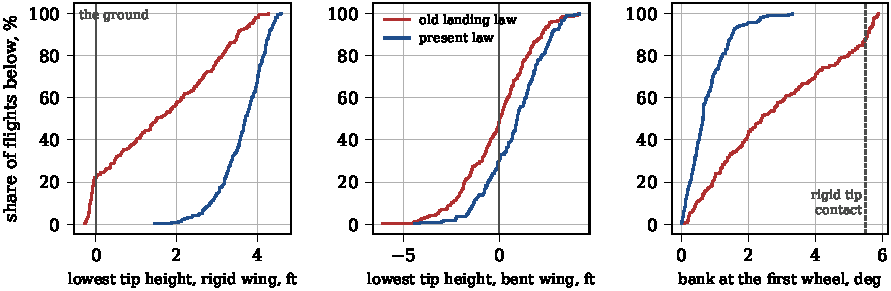
\includegraphics[width=\textwidth]{wingtips.pdf}
\caption{The confirmation set (216 flights a law): the lowest tip height from 15\,ft of wheel height to 3\,s after the first wheel for the rigid wing and with the wing's bending, and the bank at the first wheel, old landing law against present.
The dashed line is the bank at which a rigid tip touches.}\label{fig:wingtips}
\end{figure*}

\emph{The wing's bending, which doubles the problem.} The numbers above treat the wing as rigid, as the model's own tip contacts do. It is not. The wing mode of section~\ref{sec:model} puts the tips up with the lift and down with the load factor times the wing's own weight and its
fuel, so a heavy aircraft's tips are 4 ft up while it flies and droop when the lift goes. The same flights with the deflection added to the tips' height (a tip's place with the bending, not where the model's rigid contact is): at the first wheel the tips are still up (3.1 to 3.3\,ft on average), because the lift has not been dumped;
then they fall as the spoilers take the lift and the gear takes the load, to $-2.5$\,ft at 12\,450\,lb, $-4.0$ at 20\,800 and $-5.1$ at 26\,750 (medians of the lowest deflection; $-7.9$ the lowest of all), and the rigid clearance of 4.6\,ft of a calm, level landing at 26\,750\,lb is 2.1\,ft. \emph{With the bending a tip is at or below the ground
in 105 of the 216 flights under the old law and in 65 under the present one} (table~\ref{tab:roll}); by weight, 10, 39 and 56 of 72 against 1, 22 and 42 at 12\,450, 20\,800 and 26\,750\,lb. The roll loop takes the bank's share out and more than halves the count at the light weights, and it cannot take out the wing's own: the dip goes with the weight (under the present law the correlation of the tip's lowest height with weight is $-0.68$, with the
bank at the first wheel $-0.36$, with the sink $-0.20$) and a full wing is the heavy one. A low wing dips twice, once with the bank and once with its own weight. These are the model's figures from an estimate: no stiffness of the real wing is public, and the cantilever that gives these deflections is sized by strength (section~\ref{sec:model}). A stiffer wing would
dip less, and the real tips' clearance on the ground is a question for the real structure; what the study shows is that the bank is the part the laws can reach and that they now do.

\subsection{Landing across the wind: the flare's drift}\label{sec:drift}
With the bank washed out at the wheels, what is left to take the aircraft off the line in a crosswind is the flare itself. The aircraft flies the final with its nose into the wind (a crab of 4 to 22$^\circ$ here, by weight and wind). In the last 8 to 1\,ft the nose is turned onto the runway's heading, the sideslip this makes gives a side force,
and the aircraft drifts downwind. \emph{Measured.} Twelve FlightGear flights in a steady wind (the METAR wind and nothing else: no gusts, no shear), at three weights (26\,750, 19\,100 and 12\,450\,lb: full tanks, half and 1\,000\,lb of fuel) and four crosswinds (9, 19, 28 and 37\,kt at the wheels, table~\ref{tab:drift});
a steady wind makes each flight a measurement and not a draw, which the turbulent flights cannot be. The line holds within 1.6\,ft down to 15\,ft in all twelve; below it the aircraft drifts 0.5 to 7.8\,ft downwind. The drift is proportional to the crosswind and to the weight and not to the speed
(the heavy aircraft is 45\,\% faster): \emph{drift $=0.0076\times$ weight in 1\,000\,lb $\times$ crosswind in kt, in feet} (0.43\,ft rms over the twelve, 0.47 leaving each out in turn; 0.10\,ft/kt light, 0.20 full). The bench's own steady-wind sweep gave 0.12\,ft/kt at 26\,750\,lb: it had 40\,\% too little drift, which is why the bench could
not be tuned on and the flights had to be flown. \emph{The offset.} The line that the lateral loops steer to is moved upwind by the same amount, worked out in flight from the aircraft's weight and its smoothed crosswind, from 1\,000 to 700\,ft of wheel height (\texttt{ap/final-aim}). Six FlightGear flights with it on
(37 and 19\,kt, three weights): the first wheel lands $-0.5$ to $+1.9$\,ft from the line (rms 1.0\,ft) against $-0.8$ to $-6.9$\,ft without it; the bank at the first wheel and the sink are as before ($-0.3$ to $-1.1^\circ$, 0.58 to 0.71\,m/s). The aircraft realises 16\,\% more than the aim in every flight, because the wind
it smooths over the last 100 to 300\,ft is stronger than at the wheels. A coefficient 7\,\% lower would take the mean error from $+0.6$ to $+0.3$\,ft and not the spread (the rms 0.99 to 0.94\,ft, and 1.20 leaving each flight out), so it was left as measured; what is left is a weight pattern (the light flights land 1 to 2\,ft upwind) that six flights do not support a second term for.

\begin{figure}[t]\centering
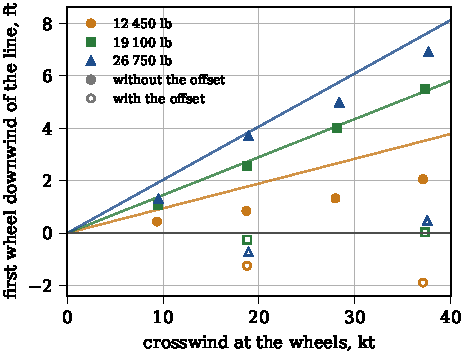
\includegraphics[width=\columnwidth]{drift.pdf}
\caption{Where the first wheel lands against the line (downwind positive), by crosswind and weight, in FlightGear's steady wind. Lines: the formula, which is also the offset's aim; filled markers: the landing without the offset (12 flights); hollow: with it (6 flights).}\label{fig:drift}
\end{figure}
\begin{table}[t]\centering\footnotesize
\begin{tabular}{@{}l r r r@{}}
\toprule
Crosswind at the wheels & 12\,450\,lb & 19\,100\,lb & 26\,750\,lb \\
\midrule
\multicolumn{4}{@{}l}{\textbf{drift from 15\,ft to the first wheel, downwind (ft)}} \\
\quad 9\,kt & 0.5 & 1.1 & 1.4 \\
\quad 19\,kt & 1.1 & 2.7 & 3.9 \\
\quad 28\,kt & 2.0 & 4.3 & 5.5 \\
\quad 37\,kt & 3.6 & 6.2 & 7.8 \\
\midrule
\multicolumn{4}{@{}l}{\textbf{touchdown error with the offset, upwind positive (ft)}} \\
\quad 19\,kt & +1.2 & +0.3 & +0.7 \\
\quad 37\,kt & +1.9 & 0.0 & $-$0.5 \\
\bottomrule
\end{tabular}

\caption{The flare's drift (downwind, from 15\,ft of wheel height to the first wheel) in twelve flights, and the touchdown error with the offset in six (upwind of the line is positive).}\label{tab:drift}
\end{table}

\emph{What it is and is not.} A steady 37\,kt across the runway is easy for this aircraft: 7.8\,ft of drift at worst, with 1$^\circ$ of bank and 0.6\,m/s of sink at the wheels. The gusty cases are the hard ones. On the 216 unseen flights the line is 5.5\,ft on average, 13\,ft at the 95th percentile and 49\,ft at worst
(12\,450\,lb in 36\,kt with severity-6 turbulence); an offset moves the mean and cannot touch the wander, and it has been tried in FlightGear only in steady wind. One thing the flights show that the offset does not touch: after the first wheel the aircraft swings upwind, 3.4 to 15.8\,ft in the first 3 to 10\,s (the 37\,kt flights 7 to 16\,ft, the
light one the most), with or without the offset, and ends the rollout 1 to 2\,ft right of the line. The decrab is not finished when the wheels touch (the nose is 3.6$^\circ$ right of the runway's heading at full weight and 11$^\circ$ at 12\,450\,lb in 37\,kt), so the aircraft rolls
out along the nose and the steering takes it back: the ground track turns 0.6 to 3.6$^\circ$ towards the nose in the first 1 to 3\,s, and the line follows. After that the nose-wheel steering, a proportional law, holds the nose 1 to 2$^\circ$ into the wind
(a steady heading error of 2 to 3$^\circ$ against the weathercock) while the wheels roll along the course. That is not the flare's drift and the offset's formula does not cover it. At the light weight it was a limit: the decrab's term was held to 10$^\circ$ of ruddervator and sat there for the last 3\,s, and an earlier start did not help (it left the nose where it was and put the line 5 to 18\,ft further out). With the limit at 20$^\circ$ in the air (laws version~4; on the ground it is 10$^\circ$ as before) the 12\,450\,lb flight in 37\,kt touches down with 4.9$^\circ$ of nose instead of 11.2$^\circ$ and 15.7$^\circ$ of sideslip instead of 10.1$^\circ$, swings 6.0\,ft instead of 15.8, and drifts no more (3.9 against 3.8\,ft), the touchdown error unchanged (+1.8\,ft). 30$^\circ$ gives the same as 20: the ruddervators' own travel, shared with the pitch, is the next limit, about 15.6$^\circ$ of sideslip, a complete decrab to about 26\,kt across at 98\,KEAS and 38\,kt at 143\,KEAS. The heavier flights are unchanged, 3.7$^\circ$ of nose at touchdown and a swing of 7 to 9\,ft: the clip does not bind there, and a higher gain trades it for 1 to 4\,ft more drift without shortening the swing. The headless regression, 20 scripts without the FlightGear phases, has the same passes and misses as before the change. An airliner, as I understand it, takes the decrab's drift out with bank within its tips' and engines' clearance and has an autoland limit below the crosswind a pilot may land in;
this wing has less to give in the bank, and so much less with its dip (section~\ref{sec:tips}), so the correction has to come from where the aircraft aims.

\subsection{Failures}\label{sec:failures}
\begin{figure*}[t]
\centering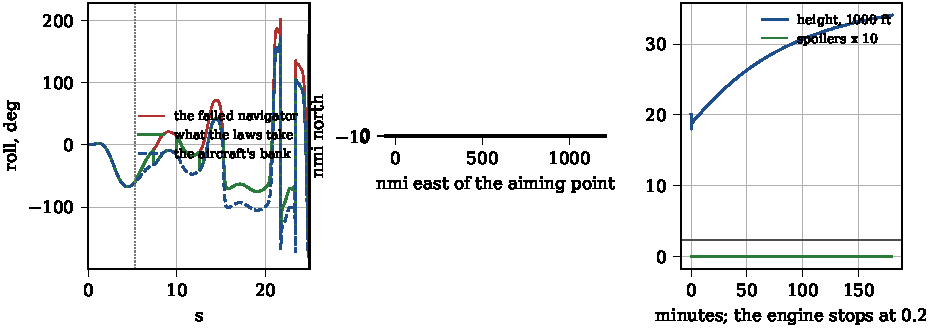
\includegraphics[width=\textwidth]{failures.pdf}
\caption{Left: one of two navigators drifts to 30$^\circ$ in roll, as in the 2017 loss; the dotted line is the miscompare flag. Middle and right: the
engine stopped at 20\,000\,ft, 30\,nmi from the field, flying away from it: the track to a landing, and height with the spoilers.}\label{fig:failures}
\end{figure*}
In 2017 an RQ-4B flying on two navigators took one's false roll and was at about 152$^\circ$ of roll 5.5\,s later \cite{aib}. With the same failure
the model's vote is out by 1.5$^\circ$ at most, until the two disagree by 3$^\circ$, and the bank stays within 0.93$^\circ$
(figure~\ref{fig:failures}). One of four jumping 60$^\circ$ does not move the vote. Both of two wrong the same way is not caught: the aircraft flies
banked 26$^\circ$ with no flag raised. No vote survives a common error, and the reference that picks between two is not checked against them.

With the uplink cut on a leg the aircraft leaves its plan 30.1\,s later and lands 24 minutes after. With the engine stopped at 20\,000\,ft, 30\,nmi
out and flying away, it turns back, burns its surplus height in a circle over the approach and touches down 1600\,ft past the aiming point at
0.89\,m/s, 21 minutes after the failure; from 50\,000\,ft and 100\,nmi the same, 47 minutes after. The model glides at 31 to 33 to 1; the planner
that chooses the runway counts on 20, and arrives with 8900 and 21\,400\,ft in hand where it expected 4700 and 13\,200. The windmilling engine's drag
is not modelled. With no runway in reach an alert is raised and nothing more: a landing off a runway is not built.

\subsection{By hand}
In the protected law, full back stick held for 30\,s takes the angle of attack 0.17 to 0.25$^\circ$ past its limit at most; full forward stick stops at
Mach~0.649 at the cruise and 179\,KCAS low down; full side stick at 13$^\circ$ of bank at the cruise and 22$^\circ$ lower. A simple pilot climbing
500\,ft and turning 30$^\circ$ ends within 6\,ft and 0.4$^\circ$ with the stick delayed by 0 and by 0.3\,s; with 1.5\,s, the order of a satellite
link's delay, he arrives but the height hunts by 84\,ft. In the direct law the Dutch roll's damping ratio is 0.29 to 0.35, against the bare airframe's
0.03 to 0.07, and a dive recovered with full back stick reaches 3.3\,$g$. The structural limits it is flagged against, 2.5\,$g$, 200\,KEAS and
Mach~0.70, are assumed: none is published.

\subsection{The station}\label{sec:station}
\begin{figure}[t]
\centering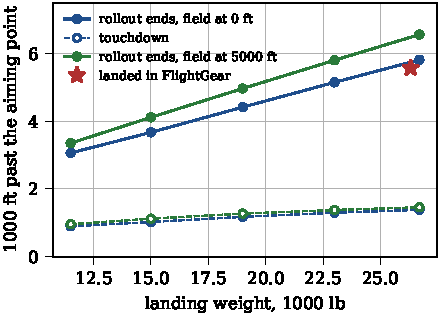
\includegraphics[width=\columnwidth]{landing_roll.pdf}
\caption{The landing's roll the station forecasts, from the flight model's own landings, and a landing made in FlightGear ten minutes after take-off.}\label{fig:roll}
\end{figure}
Flown through the station's protocol, the model taxis, takes off and joins its route on a start command, goes to a point and holds within 0.25\,nmi of
its circle, changes height in the hold, resumes its plan, refuses what it must (a go-to on the ground, a second start, 70\,000\,ft, a repeated
sequence number), and 30.0\,s after the station goes silent leaves for home. The nine alerts each rise within 0.5\,s of their cause, or 29.5\,s into a
silence, and clear with it. Control passes between stations only by offer and acceptance, or by taking it from a station that is no longer heard; a
watching station's commands and stick are refused. The plan check and the glide-reach calculation, ported from the aircraft's Python to the page, give
the same verdict on 200 damaged plans and the same reach in 50 cases.

The forecast of a 43-minute plan is 2.2\,\% long in time and 2.2\,\% short in fuel against the model's flight of it; a climb to 45\,000\,ft, 2.0 and
2.9\,\% over. The landing's roll is forecast from the model's own landings by weight (figure~\ref{fig:roll}): 3060\,ft past the aiming point at
11\,500\,lb and 5810\,ft at full weight, a tenth more at a field at 5000\,ft. A landing soon after take-off is a heavy one.

\subsection{In FlightGear}\label{sec:fgres}
\begin{figure}[t]
\centering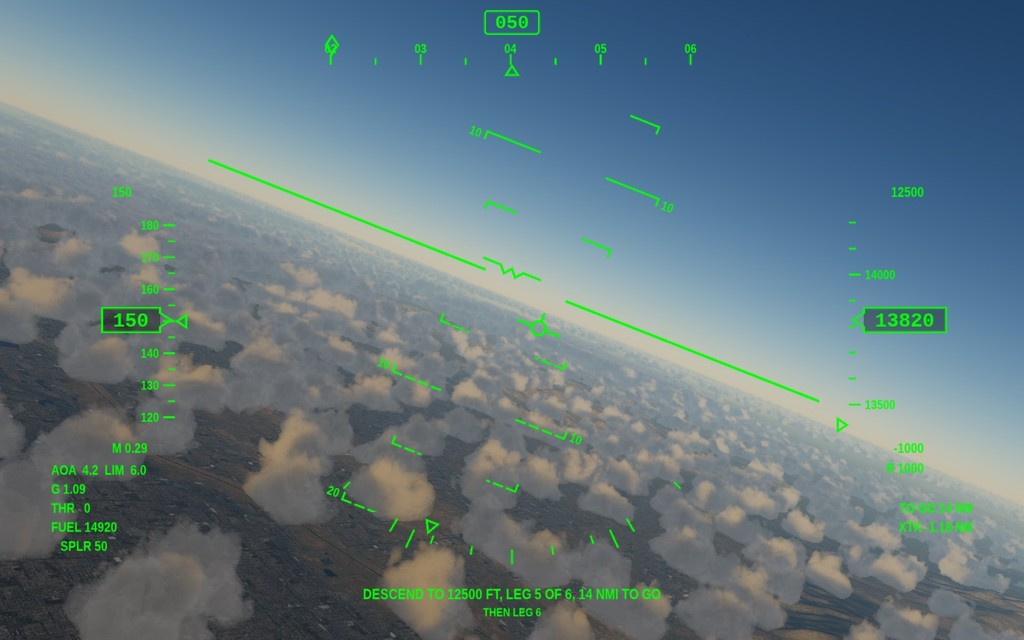
\includegraphics[width=\columnwidth]{hud.jpg}
\caption{The head-up display over the nose camera in a 22$^\circ$ banked turn in FlightGear.}\label{fig:hud}
\end{figure}
The aircraft starts on a runway in about 20\,s with the flight model at 120\,Hz and stands still for a minute. Started in the air at 20\,000\,ft and
150\,KCAS it holds its height within \the\numexpr\FgAirHHi-\FgAirHLo\relax\,ft, its speed within 0.6\,kt and its bank within \FgAirBank$^\circ$ over two minutes
(section~\ref{sec:review}, item~\ref{it:wind}). Commanded only through the link, by the scripting-language copy of the mission manager, it takes off,
joins its route, holds within 2\,\% of its circle's radius, is flown by hand and handed back, loses its link, flies the contingency route and lands;
33 of 33 commands are answered as the Python copy answers them, and the manager's events come in the same order. That landing, at 26\,320\,lb, was
down to 15\,kt \FgLandPast\,ft past the aiming point, where the flight model alone needs \FgLandModel\,ft (figure~\ref{fig:roll}).
These runs in FlightGear (phase~9 of the logs) were repeated on this version after the section's moment was corrected and the flare law rewritten:
all four phases pass (5, 10, 9 and 5 checks). The first repeat of the event-order check missed, because it read the manager's events a frame before the
manager wrote the last one (at four times speed and two frames a second); the landing itself was the same to 170\,ft, and the check now waits for the event.

The head-up display's horizon lies within \FgHudHorizon$^\circ$ of the scenery's and its figures are the aircraft's within rounding (figure~\ref{fig:hud}); it
costs no measurable frame rate. The belly camera stays within \FgCamPoint$^\circ$ of a ground point through a 149$^\circ$ turn and within \FgCamShip$^\circ$ of a
moving ship.

\subsection{Sound}
The sound is synthesised, not recorded, by the author's PyWopWop \cite{pww}: the fan and its buzz-saw tones, compressor, combustion, turbine and
jet from the engine's state, the wind on the nose, the tyres, the gear in the airflow, the touchdowns and the airframe. Recordings of the aircraft gave
the fan's blade count, 24, its speed at take-off, 8290\,rpm from the blade-passage tone and the buzz-saw's spacing less the Doppler shift, and its
idle, about 2250\,rpm. The engine's spectrum against a take-off recording is 7.5\,dB out in the root mean square over its bands, where 6 was the
limit: a miss, outside the counts of table~\ref{tab:checks} because no log holds it. The start is the running engine's loops played from the rotors'
assumed run-up; no recording of a start was found.

\section{Corrections found during validation}\label{sec:review}
The changes that the comparisons forced are listed here because each removed an inconsistency rather than tuning a coefficient.
\begin{enumerate}
\item \emph{The 3-D model's scale.} It was to be the geometry; its length and span disagree by 29\,\%. It gives shapes only, and in FlightGear it is
stretched in span outboard of the gear and squashed to the published height.
\item \emph{The flat rating.} Read as a thrust cap it gave 45\,\% too much thrust less drag at 10\,000\,ft. Read as the turbine temperature that
gives the rated thrust at rest at sea level, it gives the measured climb, unfitted.
\item \emph{The climb's energy.} The first calibration left out the energy that goes into true airspeed rising with height on the schedule, 7 to 10\,\%
of the climb rate. It showed when the laws flew the climb in time and took 6.6\,\% longer than the quasi-steady mission. With the term in and the fit
redone the lower climb rates, which had looked 1\,\% off, are 4 to 11\,\% low.
\item \emph{The landing weight.} One assumed landing weight could not explain the two approach speeds. The weights from the fuel model along each
flight do, at one lift coefficient.
\item \emph{The centre of gravity.} First put at 25 to 29\,\% of the mean chord, it left no static margin once the neutral point was computed; moved to 22\,\%.
\item \emph{The speed integral at the angle-of-attack limit.} While the limit held the nose down the speed loop's integral went on asking; released, the
first glide without the engine came down final 15\,kt slow. It holds still at the limit now.
\item \emph{The air start in FlightGear.}\label{it:wind} A start in the air swung 142 to 157\,KCAS. A table of the model's own level trims did not cure
it, and frame-by-frame records showed why: FlightGear begins the flight in a wind of 37\,kt and blends to the wind aloft over two seconds, which threw
the airspeed 20\,ft/s either way and the sideslip to 8$^\circ$. The flight model is now held until the wind has settled and then set on its trim in
that air. Where the height asked for cannot be flown with the fuel on board, fuel is taken off first.
\item \emph{The navigators' switches.} A station that connected before the flight model had loaded left the four navigators switched off: its
listeners created their switches empty and the flight model then kept them so. The laws flew without attitude and the height loop diverged. The model's
non-zero starting values are restored at the start.
\item \emph{The mission manager's two copies.} Checked command by command against each other; one difference stands, the hand-flown mode on the ground.
\item \emph{The landing that ran long.} A landing in FlightGear rolled 5900\,ft and looked like a fault. It was a landing at 26\,300\,lb; the check
had no weight in it and now compares with the flight model alone at the same weight, and the station forecasts the roll.
\end{enumerate}

\section{Assessment}\label{sec:assess}
\Nmiss{} checks miss (table~\ref{tab:misses}, on the last pages). They fall into four kinds.
\begin{itemize}
\item \textbf{A source that is not what it was taken for.} The 3-D model, which is not to scale (six misses), and the thesis table whose thrust was
asked to 2\,\%.
\item \textbf{Sources that cannot all be met.} NASA's and Northrop Grumman's heights; the family's members at 85\,\% thrust; a bare engine against an
installed one, in both engine models.
\item \textbf{Another model's own limits.} pyCycle's generic component maps at part power and its fan map past its top speed line; the reference
build, which does not carry the V-tail's incidence into its moment, so that it no longer trims at the cruise, and is not used.
\item \textbf{Real or open.} The section data's maximum lift at Mach~0.6 and Re 2 million; the wing's root chord, 16.5\,\%
over the drawing's because the chords carry the published area.
\end{itemize}
What the model reproduces of the real aircraft is its performance: the climb, unfitted to 40\,000\,ft and fitted above; the cruise-climb; the slope of
its lift curve; its take-off within 13\,\%; and its approach, from one landing to the other. Its endurance, 34.9\,h to NASA's ceiling, is what the
physics gives, not a fit: it is inside a sanity window of 29 to 35\,h and above NASA's ``31+'' and the RQ-4A's 30.4\,h record, whose reserves and payloads
are unknown, so it is not held to them.

What could not be compared at all is most of what makes a flight model: no stability derivative, mode, control power or response of the aircraft is
public, beyond lift-curve slopes of a longer-winged version. The damping in pitch and yaw differs by a factor of two to three between methods. The
centre of gravity is a choice that the one published figure contradicts. The laws are a plausible design that flies the way the records show the
aircraft flying, not the aircraft's laws: their touchdowns and rotation are numbers of the design chosen against the records, and they read true sideslip,
which the aircraft cannot measure. Estimates throughout: the mass breakdown and inertias, the fuel layout, the control surfaces and actuators, the
gear's springs, the idle thrust, the engine's rise from idle and its fall (the rise above 0.6 of its speed is fitted to one Citation~X recording), the bending, the
structural limits. Wind, turbulence and off-standard days are checked in one draw of each in the phase~11 checks, not statistically (the landings in gusts of sections~\ref{sec:gusts} to \ref{sec:drift} are flown in hundreds, in a bench's air that no real gust data
hold to). The wing's bending sets the tips' clearance at touchdown in the model and is an estimate. Not modelled: the loss of engine efficiency at low Reynolds number, the bent wing's twist, torsion and flutter, the windmilling engine, sensor and navigator
errors other than those set by a test, icing. The ground station has not been tried by anyone but its author: a test with a new operator is written,
with its pass mark, and waits for the operator's manual. This work is not connected with or endorsed by NASA, Northrop Grumman or Rolls-Royce.

\section{Conclusions}\label{sec:concl}
\begin{itemize}
\item A flight model of the Global Hawk RQ-4A, its wing 80 strips on a lifting line, its engine a cycle model of the AE~3007 family, with a bending
wing, runs in plain JSBSim at 120\,Hz, generated from published data, and flies in FlightGear.
\item With the engine's flat rating read as a turbine temperature and nothing fitted, it climbs from 10\,000 to 40\,000\,ft 4 to 11\,\% slower
than two measured flights. One drag increment and 1\,\% on the fan-speed limit hold the cruise-climb within
890\,ft over 20 hours and leave the time to 55\,000\,ft 9.0\,\% short (a miss); thrust and drag cannot be separated with the data there is.
\item Its trimmed lift-curve slope is 3\,\% over the flights' at Mach 0.52 and 16\,\% over at Mach 0.6 (a miss, from the added drag), and the second recorded approach follows from the spoilers fitted on the first.
\item Its endurance is 34.9\,h to NASA's 65\,000\,ft ceiling, and 35.1\,h without one: what the physics gives, with no fit to NASA's ``31+'' or to the
RQ-4A's 30.4\,h record, whose conditions are unknown. One fitted exponent for the section's moment, set to the tunnel's, made the bare airframe's speed mode at the cruise stable.
\item Flight laws of the author's design fly a mission from stand to stand, the two recorded landings within 5\,KEAS and half a metre a second of the
records, a navigator failure of the 2017 kind within a degree of bank, a lost link and a landing without the engine; they are held to their own
requirements, because nothing of the real laws or of the aircraft's response is public.
\item Days of $-20$ to $+30$\,K, turbulence and a 25\,kt wind are flown (one draw each): the laws hold height and bank; the airspeed cannot be held in gusts and the check that asked
it is a recorded miss; a flare that starts at a time to touchdown keeps a severe-turbulence landing at 1.3\,m/s. The engine's spool is a rate-limited lag fitted to a recording of a
Citation~X taking off. The ATTREX records' short-period peak, at 0.29\,Hz, leaves the model's static margin standing.
\item In gusts the aircraft's stabilisation of the landing lowers the hard landings in a lost headwind and a downdraught (73 to 42 of 96 flights, 46 to 31 of 72) and in a shear (47 to 30 of 48); two airliners' rules of thumb for the approach speed, as I read them,
buy margin to the angle-of-attack limit and cost sink and runway (Boeing's also the assumed structural limits), with no gain in the hard landings that can be shown (336 flights an arm, $\pm6$ points, flown twice). The low wing's tips limit the bank at touchdown: a stiffer roll loop with the bank washed out takes the rigid tip contacts
of 216 unseen flights from 48 to none and the line at the wheels from 14.6 to 5.5\,ft; with the model's estimated bending the tips still reach the ground in about a third, more at a full weight. In a steady crosswind in FlightGear the flare drifts the aircraft $0.0076$\,ft per knot
per 1\,000\,lb downwind, and an aim offset of that size lands the first wheel within 2\,ft of the line.
\item A transonic CFD run of the section, not trusted by the rule fixed for it, agrees with the tunnel that the model stalls early at Mach~0.6.
\item A ground control station in a browser commands it through FlightGear's own web server, and the aircraft's end of the link exists twice, checked
command by command.
\item Limits were set first and not moved. \Npass{} checks pass and \Nmiss{} miss, each with its cause; \NFpass{} of the passes are against flight
records and \NDpass{} against the design's own requirements.
\end{itemize}

\begin{thebibliography}{99}\small
\bibitem{ov} NASA, \emph{Global Hawk High-Altitude Long-Endurance Science Aircraft}, fact sheet FS-098, and overview briefings, NTRS 20090022147, 20110023961, 20170006086.
\bibitem{ops} NASA, \emph{NASA Flight Operations of Ikhana and Global Hawk}, NTRS 20090029219 and 20100003440.
\bibitem{upd} NASA, \emph{NASA Global Hawk: Project Update and Future Missions}, NTRS 20090001264.
\bibitem{fg} FlightGear flight simulator, \url{https://www.flightgear.org}; JSBSim, \url{https://github.com/JSBSim-Team/jsbsim}.
\bibitem{attrex} NASA Ames, Meteorological Measurement System, ATTREX campaigns 2011--2015, NASA ESPO archive, \url{https://espoarchive.nasa.gov/archive/browse/attrex}.
\bibitem{pastor} E.\ Pastor et al., \emph{Macroscopic Performance Analysis of NASA's Northrop Grumman RQ-4A}, Aerospace 5(1), 6, 2018.
\bibitem{glb} NASA 3D Resources, \emph{Global Hawk}, and the side-view drawing of the payload bays in NASA's Global Hawk briefings.
\bibitem{uthm} A thesis on transient flight analysis, Universiti Tun Hussein Onn Malaysia, 2013, table 2.4, quoting \emph{Jane's All the World's Aircraft}, 1999.
\bibitem{lrn} R.\,M.\ Hicks and S.\,E.\ Cliff, \emph{An Evaluation of Three Two-Dimensional Computational Fluid Dynamics Codes Including Low Reynolds Numbers and Transonic Mach Numbers}, NASA TM 102840, 1991.
\bibitem{xfoil} M.\,Drela, XFOIL: an analysis and design system for low Reynolds number airfoils, in \emph{Low Reynolds Number Aerodynamics}, Lecture Notes in
Engineering~54, Springer, 1989; version 6.99, built here without its display.
\bibitem{sfte} C.\,M.\ Eaton and R.\,K.\ Woolf, \emph{Flight Test Validation of the RQ-4 Block 20 Global Hawk Aerodynamic and Propulsive Models}, Society of Flight Test Engineers, 2009.
\bibitem{icao} ICAO, \emph{Aircraft Engine Emissions Databank}, rows of the AE~3007 variants.
\bibitem{ghazi} G.\ Ghazi, doctoral thesis on a Cessna Citation~X performance model, \'Ecole de technologie sup\'erieure, Montr\'eal, table 2.1.
\bibitem{rr} Rolls-Royce, \emph{AE~3007 turbofan}, data sheet.
\bibitem{easa} EASA, type-certificate data sheet IM.E.044, \emph{AE~3007 series engines}.
\bibitem{aib} U.S.\ Air Force, Accident Investigation Board report, RQ-4B T/N 07-2029, near Lone Pine, California, 21 June 2017.
\bibitem{hl} A.\ Hobbs and B.\ Lyall, \emph{Human Factors Guidelines for Remotely Piloted Aircraft System Remote Pilot Stations}, NASA, 2016.
\bibitem{nf} P.\ Sharpe, \emph{NeuralFoil}, \url{https://github.com/peterdsharpe/NeuralFoil}.
\bibitem{asb} P.\ Sharpe, \emph{AeroSandbox}, \url{https://github.com/peterdsharpe/AeroSandbox}.
\bibitem{matt} J.\,D.\ Mattingly, \emph{Elements of Propulsion: Gas Turbines and Rockets}, AIAA, 2006.
\bibitem{pyc} NASA Glenn, \emph{pyCycle}, \url{https://github.com/OpenMDAO/pyCycle}.
\bibitem{pww} \emph{PyWopWop: Aircraft Sound for Flight Simulators from First Principles}, \url{https://github.com/MrChillStorm/PyWopWop}.
\end{thebibliography}
\clearpage
\onecolumn
\begingroup\footnotesize
\begin{longtable}{@{}>{\raggedright\arraybackslash}p{4.9cm}>{\raggedright\arraybackslash}p{2.9cm}>{\raggedright\arraybackslash}p{9.2cm}@{}}
\caption{The \Nmiss{} misses and their causes.}\label{tab:misses}\\
\toprule
Check & Group & Cause \\
\midrule
\endfirsthead
\toprule
Check & Group & Cause \\
\midrule
\endhead
\midrule
\multicolumn{3}{r}{\emph{continued on the next page}}\\
\endfoot
\bottomrule
\endlastfoot
V1 C1 fuel flow at ICAO 85 \% thrust, kg/s  0.2858  0.2689  +6.3  5 & Engine & The C1 is modelled as a lower rating of the A2's hardware; the two variants' own databank rows differ by more than the limit at part power. \\
V5 TSFC at 45,000 ft, M 0.564, lb/h/lbf  0.5653  0.6225  -9.2  8 & Engine & A bare engine against the Citation X's installed one (bleed and power extraction); pyCycle's bare engine is 10.6 \% under the same figure. The installation factor on fuel comes from this difference. \\
V6b thrust at 43,835 ft at the fitted limit, lbf  1382  1335  +3.5  2 & Engine & After the fan-speed limit was fitted to the 45,000 ft row; the thesis's table is not exact to the 2 \% asked of it. \\
X0b A2 fuel flow at ICAO 85 \% thrust, lb/h  2876  3079  -6.6  5 & Engine against pyCycle & pyCycle's generic component maps at part power; the cycle model of the report is within 1.2 \% of the same row. \\
X1b C1 takeoff as a rating: pressure ratio  15.66  16.58  -5.6  5 & Engine against pyCycle & Generic compressor maps run at the C1's lower rating. \\
X2a TSFC at 1,500 ft, M 0.234, lb/h/lbf  0.4483  0.5309  -15.6  8 & Engine against pyCycle & A bare engine against an installed one, and generic maps at low altitude part power: about 10 \% of model uncertainty there. \\
X2b TSFC at 45,000 ft, M 0.564, lb/h/lbf  0.5562  0.6225  -10.6  8 & Engine against pyCycle & A bare engine against an installed one, as V5: both bare models are about 10 \% under the installed engine. \\
X3 fan corrected speed, 45,000 ft over 1,500 ft  1.462  1.258  +16.2  5 & Engine against pyCycle & pyCycle's generic fan map, run at 118 \% of its top speed line. \\
3-D model scaled by span: length, ft  measured  57.11  44.40  +28.6  1.0 & Geometry and mass & NASA's 3-D model is an artist's model, not to scale: scaled to the span it is 29 \% too long. It gives planform shape and widths only (its tail dihedral, 47.1 deg from the raw slope, was replaced by the published 50 deg that two head-on photographs confirm); lengths and heights come from NASA's side-view drawing. \\
3-D model scaled by span: height, ft  measured  20.78  15.20  +36.7  3.0 & Geometry and mass & As above: the 3-D model is not to scale. \\
3-D model scaled by span: wing area, ft2  measured  597.80  540.00  +10.7  3.0 & Geometry and mass & As above: the 3-D model is not to scale. \\
3-D model scaled by length: span, ft  measured  90.34  116.20  -22.3  1.0 & Geometry and mass & As above: scaled to the length its span is 22 \% short. \\
3-D model scaled by length: height, ft  measured  16.15  15.20  +6.2  3.0 & Geometry and mass & As above; the FlightGear model is squashed to the published 15.2 ft. \\
3-D model, span by span and chords by length: wing area, ft2  measured  464.70  540.00  -13.9  3.0 & Geometry and mass & As above; the wing's chords are a fit to the published 540 ft2. \\
side view: height, ft (NASA 15.2)  measured  14.34  15.20  -5.6  3.0 & Geometry and mass & NASA gives 15.2 ft and Northrop Grumman 14.6 ft; the drawing, scaled by the length, gives 14.3 ft, inside the limit of the second and outside that of the first. \\
wing as built: root chord with fillet against the side view, ft  measured  8.85  7.59  +16.5  5.0 & Geometry and mass & The wing as built keeps the 3-D model's root fillet (8.85 ft) where the drawing and photographs show 7.59 ft; with the drawing's chords the area falls short of the published 540 ft2. Open. \\
B3x fuel flow at it with 20 kW taken off, at 10000 ft, Mach 0.27: change, \%  -0.47178  -0.51432  +8.27\%  2.0 & JSBSim model as generated & The limit, 2 \% of the change, was written for changes of the size of the thrust's; the fuel flow's change at maximum thrust there nets two opposite effects out to -0.5 \%, and the 0.04 points of the fuel flow itself by which the tables' interpolation in Mach number differs from the cycle's are 8 \% of it. Kept as a miss; the limit was not changed. \\
B5 ref build trims at cruise & JSBSim model as generated & AeroSandbox's build-up does not carry a V-tail panel's twist into its pitching moment: 3 deg of tail incidence moves its moment by 0.0005, where the strip model's tail moves it by 0.11 (fdm/aero\_ref.py; a rotated section was tried and moved it by 0.008). The reference build therefore lacks the tail incidence the calibration set, and at the cruise needs 13 deg of ruddervator and nearly all the thrust. Its comparison with the strip model was made before and stands; the build is not used further. \\
S3 section maximum lift, Mach 0.6, Re 2 million  1.198  1.423  -15.8  10 & Section data and lift curve & The section data stops at 1.20, where its correction puts a shock stall; the tunnel reached 1.42. XFOIL cannot say: it does not converge past the first sonic point at Mach 0.6. A fit was made (fdm/cfd/stall\_fit.py: the tunnel's maximum lift with the CFD's shape) and met S3, but its blend back to the table's own deep stall after the CFD's last angle (10 to 12 deg) falls 0.26 to 0.37 per degree against the CFD's steepest 0.13, so by the rule written with it, it was withdrawn and the miss stays (docs/PLAN.md). The model stalls early at cruise Mach numbers, on the safe side for the laws' angle-of-attack limit. \\
A1 trimmed lift-curve slope, Mach 0.59 to 0.62, per deg  0.1341  0.1161  +15.5  10 & Section data and lift curve & From the added drag and not from a changed wing: the check trims six weights at 57,293 ft, and with the CFD's wave drag the three heaviest (21,254 lb and over) no longer hold height at full throttle, so the slope is fitted to the three lightest, 0.1341 against 0.1226 from four before. Taking the wave drag out brings it back to +5.6 \%; taking the stall fit or the tail angle out does not. It reflects a ceiling about 500 ft low at heavy weights (the mission's cruise-climb heights), inside their limit. \\
P1 time from 10,000 to 55,000 ft, s  4181.9  4595.6  -9.0 \%  5 \% & Climb, cruise-climb, endurance & The CFD's wave drag at Mach 0.55 to 0.7 was added to the section data and the drag increment refitted, 0.00586 to 0.00355 (below the 0.0040 to 0.0075 band written beforehand) and, after the tail's and the gear's lateral positions were measured, to 0.00308, fan-speed factor 1.01. One increment and one factor cannot hold the 40,000 to 55,000 ft climb rates (+11.1 and +15.6 \%), the cruise-climb heights and the total time together: the fit's compromise leaves the time 9.0 \% short against a limit of 5 (at 0.00355 the time passed, -0.1 \%, and the 737 minute height missed by 130 ft). No further fit: the limits allowed the one for each change (docs/PLAN.md, ''Wave drag from the CFD'', ''Lateral dimensions''). \\
A10 climb 10,000 to 55,000 ft hands off & Flight laws & The same climb time as the mission's P1: 4077 s flown by the laws against the quasi-steady 4452 s (-8.4 \%, limit 5), the refit's compromise between the 40,000 to 55,000 ft climb rates and the total time. It passed before the wave drag went in (4386 s, -1.5 \%). \\
O2 time from 10,000 to 55,000 ft (pressure) grows with the temperature & Off the design conditions: days, wind, turbulence & The limit was wrong, and is kept. Above FL220 the schedule is in Mach number (rising to 0.60 at 55,000 ft), so the climb rate goes with the true airspeed, which falls with the cold, while thrust and drag both go with pressure: the model's -20 K day is 3 \% slower (3,115 s against 3,021 s), and the hot days slower still (their service ceilings are about 55,000 ft at +15 K and 52,500 ft at +30 K). \\
W1 cruise in turbulence at 60,000 ft, severity 5 (sigma\_w 2.01 m/s): airspeed within 5 kt & Off the design conditions: days, wind, turbulence & The airspeed varies by the gust itself: the gust along the heading varies by 25 kt and the airspeed by 11, about half; no loop holds the airspeed within 5 kt in air that moves like this. The limit asked for what the air does not allow; height and bank, which the laws can hold, pass. \\
W1 cruise in turbulence at 60,000 ft, severity 5 (sigma\_w 2.01 m/s): load factor 0.7 to 1.3 & Off the design conditions: days, wind, turbulence & The lowest load factor in the severity-5 turbulence at 60,000 ft is 0.70 at the limit's edge (0.71 before): the 50 degree tail and the added drag leave a little less pitch stiffness in the thin air. Borderline, not a loss of control; no law's number was changed to pass it. \\
W1 cruise in turbulence at 20,000 ft, severity 3 (sigma\_w 1.11 m/s): airspeed within 5 kt & Off the design conditions: days, wind, turbulence & As at 60,000 ft: the gust along the heading varies by 15 kt, the airspeed by 11. \\
W2 mission, 25 kt wind, light turbulence: enroute: track within 0.25 nmi for 95 \% of the route & Off the design conditions: days, wind, turbulence & 94 \% against 95 \%, in a 25 kt wind from the runway heading, which is a crosswind or a tailwind on the legs, with light turbulence; phase 7b's own rule (80 \%) passes, and calm air gives 96 \%. The track loop's lookahead is 15 s. \\
\bottomrule

\end{longtable}
\endgroup
\end{document}
